\definecolor{c05p1blue}{HTML}{2A78D6}
\definecolor{c05p1orange}{HTML}{EB6834}
\definecolor{c05p1aqua}{HTML}{1BAF7A}
\definecolor{c05p1gray}{HTML}{52514E}

\section{Demand Systems in Product Space}\label{sec:05-productspace}

A \emph{demand system} gives the quantity of every good as a function of all prices and of the consumer's
budget. This chapter studies demand systems written in \emph{product space}. Each good has its own
parameters, and the model states directly how the demand for one good responds to the price of another.
The workhorse is the Almost Ideal Demand System of \citet{DeatonMuellbauer1980a}. We follow that literature
and index goods by $i$, $j$ and $k$, with $J$ goods in total. Elsewhere in the book the letter $i$ indexes
consumers. In this chapter households are indexed by $h = 1, \dots, H$, and \cref{sec:05-conventions}
collects the remaining conventions.

\subsection{Questions a demand system answers}\label{sec:05-questions}

Demand systems serve two kinds of questions. \emph{Positive} questions ask what will happen. How do
consumers substitute among goods when one price rises? How will prices respond to a merger, a tax or the
withdrawal of a product? Will a change in the rules alter the incentives of firms to invest in research and
development? \emph{Normative} questions ask whether the change is desirable. Who wins and who loses? Could
the winners compensate the losers? How large is the total compensating or equivalent variation, the money
measure of welfare change defined in \cref{sec:05-cv-ev}?

A second distinction concerns timing. \emph{Prospective} analysis predicts the effects of a policy before it
is implemented. Because the policy has not yet generated data, prospective analysis needs a model of demand
and supply, and sometimes a model of dynamic investment as well. \emph{Retrospective} analysis measures what
happened after a policy was implemented. It relies on causal identification from the variation that the
policy created. The two approaches complement each other. Only a model can evaluate a policy that has never
been tried, and only retrospective evidence can tell us whether a model predicted well.

One policy question runs through this chapter. The Agreement on Trade-Related Aspects of Intellectual
Property Rights (TRIPS) requires members of the World Trade Organization to enforce product patents in all
fields of technology, including pharmaceuticals. Countries that excluded pharmaceuticals from product patents
were given a transition period to amend their laws. Between April 1972 and March 2005, India recognized only
process patents for pharmaceuticals \citep{ChaudhuriGoldbergJia2006}, and Indian firms sold their own
versions of molecules patented abroad. Enforcing patents would remove
these domestic versions from the market. Would consumers then buy the foreign version of the same molecule,
a different domestic molecule, or nothing in the segment? How much would prices rise, and how would the loss
to consumers compare with the gain to patent holders? \Cref{sec:05-cgj} studies the prospective answer of
\citet{ChaudhuriGoldbergJia2006}, which is built on the demand system of this chapter. \Cref{sec:05-dgg}
confronts it with the retrospective evidence of \citet{DugganGarthwaiteGoyal2016}.

\subsection{Why microfoundations}\label{sec:05-microfoundations}

A \emph{microfounded} demand system is derived from an explicit model of optimizing consumers. It has three
advantages over a purely statistical description of demand. The first is internal consistency. The budget
constraint holds, demands do not change when all prices and income scale up together, and the cross-price
effects obey the symmetry restrictions derived in \cref{sec:05-duality}. The second is that the model rests
on \emph{primitives}, preferences and technology, which we can treat as invariant to the policy under study.
Reduced-form coefficients estimated under one policy regime need not survive a change of regime. The third
is that the model links observed behavior to the primitives through an assumption about behavior, here
utility maximization. Observed choices then reveal preferences.

These properties deliver the two products we want from a demand model. Policy-invariant primitives permit
prospective analysis, because we can solve the model again under the new policy. The link to preferences
permits normative statements, because the expenditure function converts a change in prices into a money
measure of welfare.

A statistical demand system can fit the data well and still fail these tests. Consider the \emph{double-log}
system, in which every log quantity is linear in log prices and log income with constant elasticities. It is
a natural first regression, and it imposes no theory at all. The next proposition shows how little of it
survives the budget constraint.

\begin{proposition}[Double-log demand and the budget constraint]\label{prop:05-loglinear}
Suppose that for every good $i$ and every $(p, I) \in \R^J_{++}\times\R_{++}$,
\begin{equation}\label{eq:05-loglinear}
\ln q_i = a_i + \sum_{j=1}^J e_{ij}\ln p_j + \eta_i\ln I ,
\end{equation}
with constant coefficients $a_i$, $e_{ij}$ and $\eta_i$, and that the budget identity $\sum_i p_iq_i = I$
holds everywhere. Then $\eta_i = 1$, $e_{ii} = -1$, $e_{ij} = 0$ for $j \neq i$, and $\sum_i e^{a_i} = 1$.
The only double-log system that satisfies the budget constraint at all prices and incomes is the
Cobb-Douglas demand system.
\end{proposition}

\begin{proof}
Divide the budget identity by $I$ and substitute \eqref{eq:05-loglinear}:
\begin{equation*}
\sum_{i=1}^J \exp\Big(a_i + \sum_{j=1}^J\big(e_{ij} + \indic(i=j)\big)\ln p_j + (\eta_i - 1)\ln I\Big) = 1 .
\end{equation*}
Write $x = (\ln p_1, \dots, \ln p_J, \ln I)^\T$, which ranges over all of $\R^{J+1}$. Term $i$ equals
$e^{a_i}\exp(\ell_i^\T x)$ for a coefficient vector $\ell_i$. Collect the terms that share the same vector,
and move the constant 1 to the left side as the term $-\exp(0^\T x)$. Exponentials of distinct linear forms
are linearly independent functions on $\R^{J+1}$. To see this, restrict them to a line on which the distinct
forms have distinct slopes, and use the independence of $e^{\lambda_1 t}, \dots, e^{\lambda_m t}$ for
distinct $\lambda$'s. Every coefficient of the collected sum must therefore vanish. The coefficient of a
group with $\ell \neq 0$ is a sum of positive numbers $e^{a_i}$, so no such group can exist. Hence
$\ell_i = 0$ for every $i$, and the coefficient of the zero form gives $\sum_i e^{a_i} = 1$. The condition
$\ell_i = 0$ reads $e_{ij} + \indic(i=j) = 0$ and $\eta_i = 1$.
\end{proof}

The double-log system remains useful as a local approximation, and we meet it again at the upper levels of
multi-level demand systems in \cref{sec:05-hlz}. As a global model it cannot satisfy the budget constraint,
its elasticities need not obey the restrictions of consumer theory, and it delivers no welfare measure. The
systems in the rest of this chapter are built so that they do all three.

\subsection{Product space and characteristic space}\label{sec:05-ps-vs-cs}

\Cref{ch:diffprod} introduced the two ways of modeling demand for differentiated products. In \emph{product
space}, preferences are defined over the goods themselves, and demand is written as
\begin{equation}\label{eq:05-productspace}
q_i = f_i(p_1, \dots, p_J, I), \qquad i = 1, \dots, J,
\end{equation}
with parameters indexed by goods. In \emph{characteristic space}, goods are bundles of characteristics and
preferences are defined over the characteristics. The number of parameters then grows with the number of
characteristics and with the dimension of consumer heterogeneity, rather than with the number of goods.

Product space is the more natural starting point. Substitution patterns are estimated from the data instead of
being imposed by the location of goods in a space of attributes. Goods can be complements as well as substitutes. No data on
characteristics are needed, which helps when the relevant attributes are hard to measure, as for books or
films.

Its central problem is dimensionality. Even a linear system $q = a + Ap$ has $J^2$ price coefficients in the
matrix $A$, which is 10{,}000 coefficients for $J = 100$ goods. Theory helps but not enough. In the Almost
Ideal Demand System, symmetry, homogeneity and adding up leave $\frac{J(J-1)}{2}$ free price coefficients
(\cref{sec:05-aids-limits}), which is still 4{,}950 for $J = 100$. Dimensionality has two further costs. Each
of the $J$ prices is a potentially endogenous regressor in every equation, so estimation requires
instruments that move the prices independently of one another (\cref{sec:05-estimation}). And because every
parameter belongs to a particular good, the model cannot predict demand for a good that has never been sold.

There are two remedies. The first aggregates goods into a few groups and assumes that consumers budget in
stages, so that each stage involves only a few goods. The theory of separability that justifies this
procedure is developed in \cref{sec:05-separability}, and the applications of \citet{HausmanLeonardZona1994}
and \citet{ChaudhuriGoldbergJia2006} take this route. The second remedy moves to characteristic space, as
in \cref{ch:discrete,ch:logit,ch:blp}. Its costs are data on characteristics, more complex estimation, and
restrictions on substitution that come from the structure of the random utility model.

\subsection{Three product-space systems}\label{sec:05-three-systems}

We now compare three systems that are all derived from a model of consumer behavior. The logit and the
constant elasticity of substitution (CES) systems place all substitution in a single parameter. The Almost
Ideal Demand System frees the cross effects. \Cref{ch:diffprod,ch:logit} develop the first two in depth, so
the derivations here are brief.

\casehead{Logit}
A population of $M$ consumers, indexed by $h$, each buys one unit of one of the goods $i = 1, \dots, J$ or
of an outside good $i = 0$. Consumer $h$ obtains utility
\begin{equation*}
u_{hi} = \delta_i - \alpha p_i + \epsilon_{hi}, \qquad u_{h0} = \epsilon_{h0},
\end{equation*}
where the $\epsilon_{hi}$ are independent type-I extreme value draws. In this subsection only, $\delta_i$
is a taste shifter that excludes price, and $\alpha > 0$ is the logit price coefficient. (Elsewhere in the
book $\delta$ denotes mean utility including price, and in the Almost Ideal Demand System $\alpha_i$ is an
intercept.) The share of consumers who choose good $i$ and the share who choose the outside good are
\begin{equation*}
s_i = \frac{e^{\delta_i - \alpha p_i}}{1 + \sum_{k=1}^J e^{\delta_k - \alpha p_k}}, \qquad
s_0 = \frac{1}{1 + \sum_{k=1}^J e^{\delta_k - \alpha p_k}},
\end{equation*}
as \cref{ch:discrete} derives from the extreme value distribution. The ratio of the two is
$\frac{s_i}{s_0} = e^{\delta_i - \alpha p_i}$. Quantities are $q_i = Ms_i$, so the market size $M$ cancels
from the ratio $\frac{q_i}{q_0}$. Taking logs gives the market-level logit,
\begin{equation}\label{eq:05-logit}
\ln q_i - \ln q_0 = \delta_i - \alpha p_i .
\end{equation}
The left side is computed from data, and the right side is linear in the parameters. Once we add an error
term to $\delta_i$, the logit can be estimated by linear regression \citep{Berry1994}, as \cref{ch:logit}
explains. Differentiating the shares gives $\frac{\partial s_i}{\partial p_i} = -\alpha s_i(1-s_i)$ and
$\frac{\partial s_i}{\partial p_k} = \alpha s_is_k$ for $k \neq i$. The elasticities are therefore
\begin{equation}\label{eq:05-logit-elast}
\varepsilon_{ii} = -\alpha p_i(1 - s_i), \qquad \varepsilon_{ik} = \alpha p_ks_k \quad (k \neq i).
\end{equation}
The cross elasticity with respect to $p_k$ is the same for every good $i$. When good $k$ raises its price,
all other goods gain demand in the same proportion, however close or distant they are to $k$. This is the
independence of irrelevant alternatives, studied in \cref{ch:logit}.

\casehead{Constant elasticity of substitution}
A single consumer with budget $I$ has CES utility. The next proposition collects the facts we use. In this
chapter $\sigma$ denotes the elasticity of substitution. Elsewhere in the book it denotes the nesting
parameter of the nested logit.

\begin{proposition}[CES demand]\label{prop:05-ces}
Let $U(q) = \big(\sum_{j=1}^J a_j^{\frac{1}{\sigma}}q_j^{\frac{\sigma-1}{\sigma}}\big)^{\frac{\sigma}{\sigma-1}}$
with $a_j > 0$, $\sigma > 0$ and $\sigma \neq 1$, and let the consumer maximize $U$ subject to
$\sum_j p_jq_j = I$. Define the CES price index
$P^{CES} = \big(\sum_{j=1}^J a_jp_j^{1-\sigma}\big)^{\frac{1}{1-\sigma}}$. Then:
\begin{enumerate}[label=(\roman*)]
\item Demand is $q_i = a_i\big(\frac{p_i}{P^{CES}}\big)^{-\sigma}\frac{I}{P^{CES}}$, and the budget share is
  $w_i = \frac{p_iq_i}{I} = a_i\big(\frac{p_i}{P^{CES}}\big)^{1-\sigma}$.
\item Indirect utility is $v(p, I) = \frac{I}{P^{CES}}$ and the expenditure function is $e(p, u) = P^{CES}u$,
  so preferences are homothetic.
\item The Marshallian elasticities are $\varepsilon_{ii} = -\sigma + (\sigma - 1)w_i$,
  $\varepsilon_{ik} = (\sigma - 1)w_k$ for $k \neq i$, and the expenditure elasticity is $\eta_i = 1$.
\end{enumerate}
\end{proposition}

\begin{proof}
Write $U = S^{\frac{\sigma}{\sigma-1}}$ with $S = \sum_j a_j^{\frac{1}{\sigma}}q_j^{\frac{\sigma-1}{\sigma}}$.
By the chain rule,
\begin{equation*}
\frac{\partial U}{\partial q_i} = \frac{\sigma}{\sigma-1}S^{\frac{1}{\sigma-1}}\cdot
\frac{\sigma-1}{\sigma}a_i^{\frac{1}{\sigma}}q_i^{-\frac{1}{\sigma}}
= U^{\frac{1}{\sigma}}a_i^{\frac{1}{\sigma}}q_i^{-\frac{1}{\sigma}},
\end{equation*}
because $S^{\frac{1}{\sigma-1}} = U^{\frac{1}{\sigma}}$. The first-order condition
$\frac{\partial U}{\partial q_i} = \lambda p_i$ gives $q_i = a_iU(\lambda p_i)^{-\sigma}$. Substitute into
the budget constraint:
\begin{equation*}
I = \sum_j p_jq_j = U\lambda^{-\sigma}\sum_j a_jp_j^{1-\sigma} = U\lambda^{-\sigma}(P^{CES})^{1-\sigma}.
\end{equation*}
Hence $U\lambda^{-\sigma} = I(P^{CES})^{\sigma-1}$, and
$q_i = a_ip_i^{-\sigma}I(P^{CES})^{\sigma-1} = a_i\big(\frac{p_i}{P^{CES}}\big)^{-\sigma}\frac{I}{P^{CES}}$.
Multiplying by $\frac{p_i}{I}$ gives the share. For (ii), substitute the demands into $S$:
\begin{equation*}
S = \sum_j a_j^{\frac{1}{\sigma}}a_j^{\frac{\sigma-1}{\sigma}}\Big(\frac{p_j}{P^{CES}}\Big)^{1-\sigma}
\Big(\frac{I}{P^{CES}}\Big)^{\frac{\sigma-1}{\sigma}}
= \Big(\frac{I}{P^{CES}}\Big)^{\frac{\sigma-1}{\sigma}}\sum_j a_j\Big(\frac{p_j}{P^{CES}}\Big)^{1-\sigma}
= \Big(\frac{I}{P^{CES}}\Big)^{\frac{\sigma-1}{\sigma}} ,
\end{equation*}
since the last sum equals one by the definition of $P^{CES}$. Then $v = S^{\frac{\sigma}{\sigma-1}} =
\frac{I}{P^{CES}}$, and inverting $u = \frac{e}{P^{CES}}$ gives $e(p,u) = P^{CES}u$. For (iii), take logs of
the demand function, $\ln q_i = \ln a_i - \sigma\ln p_i + (\sigma - 1)\ln P^{CES} + \ln I$. Differentiating
$\ln P^{CES} = \frac{1}{1-\sigma}\ln\sum_k a_kp_k^{1-\sigma}$ gives
$\frac{\partial\ln P^{CES}}{\partial\ln p_j} = \frac{a_jp_j^{1-\sigma}}{\sum_k a_kp_k^{1-\sigma}} = w_j$.
Hence $\varepsilon_{ij} = -\sigma\indic(i=j) + (\sigma - 1)w_j$ and $\eta_i = 1$.
\end{proof}

Writing $a_j = e^{\sigma\delta_j}$, with $\delta_j$ a taste shifter, the log of the demand function takes the
form
\begin{equation}\label{eq:05-ces}
\ln q_i = \sigma\Big(\delta_i - \ln\frac{p_i}{P^{CES}}\Big) + \ln\frac{I}{P^{CES}} .
\end{equation}
The normalization $\sum_j e^{\sigma\delta_j} = 1$ makes $P^{CES} = \bigl(\sum_j a_j\bigr)^{\frac{1}{1-\sigma}} = 1$
when all prices equal one. The parameter $\sigma$ is the elasticity of substitution.
From part (i), $\ln\frac{q_i}{q_k} = \ln\frac{a_i}{a_k} - \sigma\ln\frac{p_i}{p_k}$, so a one percent rise in
the relative price $\frac{p_k}{p_i}$ raises the relative quantity $\frac{q_i}{q_k}$ by $\sigma$ percent.
Goods are gross substitutes when $\sigma > 1$. The cross elasticity $(\sigma-1)w_k$ does not depend on $i$,
so the CES has the same proportional substitution as the logit. The compensated cross elasticity, obtained
from the Slutsky equation of \cref{sec:05-elasticity-identities}, is $\sigma w_k$.

\casehead{The Almost Ideal Demand System}
The third system expresses the budget share of each good as
\begin{equation}\label{eq:05-aids-preview}
w_i = \alpha_i + \sum_{j=1}^J\gamma_{ij}\ln p_j + \beta_i\ln\frac{I}{\mathbf{P}} ,
\end{equation}
where $w_i = \frac{p_iq_i}{I}$ and $\mathbf{P}$ is a price index defined in \cref{sec:05-aids}. Shares
respond to every log price through a separate coefficient $\gamma_{ij}$, and to log real expenditure
$\ln\frac{I}{\mathbf{P}}$ through $\beta_i$. \Cref{sec:05-aids} derives the system from an expenditure
function.

\begin{table}[htbp]
\centering
\caption{Three product-space demand systems compared}\label{tab:05-three-systems}
\footnotesize
\begin{tabularx}{\textwidth}{>{\raggedright\arraybackslash}p{2.55cm}
  >{\raggedright\arraybackslash}X >{\raggedright\arraybackslash}X >{\raggedright\arraybackslash}X}
\toprule
 & Logit (market level) & CES & AIDS \\
\midrule
Dependent variable & $\ln q_i - \ln q_0$ & $\ln q_i$ (or share $w_i$) & budget share $w_i$ \\
\addlinespace
Substitution parameters & one ($\alpha$) & one ($\sigma$) & $\frac{J(J-1)}{2}$ free $\gamma_{ij}$ \\
\addlinespace
Level parameters & $J$ taste shifters $\delta_i$ & $J - 1$ free $\delta_i$ & $2(J-1)$ free $\alpha_i$,
  $\beta_i$, and $\alpha_0$ \\
\addlinespace
Own elasticity $\varepsilon_{ii}$ & $-\alpha p_i(1 - s_i)$ & $-\sigma + (\sigma - 1)w_i$ &
  $-1 + \frac{1}{w_i}\frac{\partial w_i}{\partial\ln p_i}$, \eqref{eq:05-elast-marshall} \\
\addlinespace
Cross elasticity $\varepsilon_{ik}$ & $\alpha p_ks_k$, the same for all $i$ & $(\sigma - 1)w_k$, the same
  for all $i$ & $\frac{1}{w_i}\frac{\partial w_i}{\partial\ln p_k}$, any sign \\
\addlinespace
Engel curves & no income effects (each consumer buys one unit) & homothetic, $\eta_i = 1$ & shares linear
  in $\ln I$, luxuries and necessities \\
\addlinespace
Choke (virtual) price & infinite & infinite & finite if the own share falls with price ($\gamma_{ii} < 0$
  when $\beta_i = 0$) \\
\addlinespace
Aggregation & exact: shares add up individual discrete choices & representative consumer with homothetic
  preferences & almost exact: representative budget level $I_0$ \\
\addlinespace
Typical data & shares of many products, with an outside good & expenditure on many varieties & budget
  shares of a few goods or groups over time or markets \\
\bottomrule
\end{tabularx}
\par\smallskip
\begin{minipage}{\textwidth}\footnotesize
Notes: Elasticities are signed. In the logit column $s_i$ is the market share including the outside good. In
the CES and AIDS columns $w_i$ is the budget share. The AIDS count of free $\gamma_{ij}$ imposes adding up,
homogeneity and symmetry (\cref{sec:05-aids-limits}). Aggregation for AIDS is developed in
\cref{sec:05-aggregation}.
\end{minipage}
\end{table}

\Cref{tab:05-three-systems} sets the three systems side by side. The logit and the CES buy parsimony with
restrictive substitution, because one parameter governs every cross effect. Consumers who leave a product
spread over the other products in proportion to their sizes, whatever the attributes of those products. The AIDS frees the cross
effects at the cost of many parameters.

The row on choke prices matters for welfare. A \emph{choke price}, or \emph{virtual price}, is the price at
which the demand for a good falls to zero \citep{Hicks1940,Rothbarth1941}. Removing a good from the market
is equivalent, for consumers, to raising its price to the virtual price. Under CES and logit the demand for
a good stays positive at every finite price, because $p_i^{-\sigma}$ and $e^{-\alpha p_i}$ never reach
zero. The virtual price is infinite, and the welfare loss from removing a good depends only on its share and
on the single substitution parameter. The value of variety is then built into the functional form. Under
the AIDS the share is linear in $\ln p_i$ when $\beta_i = 0$ and quadratic otherwise. When it falls with the
own price, it reaches zero at a finite price, so the loss depends on the estimated own and cross effects.
\Cref{sec:05-welfare-virtual} develops this comparison.

\subsection{Conventions for this chapter}\label{sec:05-conventions}

Goods are indexed by $i, j, k = 1, \dots, J$, and in this chapter the $J$ goods exhaust the budget under
study. Households are indexed by $h = 1, \dots, H$ and appear as subscripts, as in $I_h$ and $w_{ih}$. The
Hicksian demand $h_i(p, u)$ (defined in \cref{sec:05-ump-emp}) is always written with its arguments, so it cannot be confused with a household
index. Total expenditure, which we also call income, is $I$, and the budget share of good $i$ is
$w_i = \frac{p_iq_i}{I}$. Logarithms are natural logarithms.

Elasticities are signed throughout this chapter, as in the tables of the papers we study. The Marshallian
price elasticity is $\varepsilon_{ij} = \frac{\partial\ln q_i}{\partial\ln p_j}$, so own-price elasticities
are negative. This departs from the convention elsewhere in the book, where the own-price elasticity is
reported as a positive number. The Hicksian elasticity is $\varepsilon^h_{ij}$ and the expenditure
elasticity is $\eta_i$. The Slutsky matrix is $S = [S_{ij}]$ (\cref{sec:05-slutsky}), and we reserve $s$ for market shares. We write
the indicator $\indic(i = j)$ instead of a Kronecker delta, because $\delta$ denotes mean utility elsewhere
in the book. Additive errors in share equations are written $\xi$, while the papers often write
$\varepsilon$, which here denotes an elasticity.

\section{Consumer Duality: The Toolkit}\label{sec:05-duality}

This section collects the results of consumer theory that we need to derive, restrict and use the AIDS.
We keep the argument self-contained and prove every result we use. \Cref{app:math} restates these results for
reference and adds producer duality and integrability. The treatment parallels \citet[ch.~2]{DeatonMuellbauer1980b}. They develop the cost
function in \S 2.3 (pp.~37--42), the properties of demands in \S 2.4 (pp.~43--46) and duality in \S 2.5
(pp.~47--50). Their $c(u, p)$ is our $e(p, u)$, and their $x$ is our total expenditure $I$.

\subsection{Utility maximization and expenditure minimization}\label{sec:05-ump-emp}

\begin{assumption}[Preferences]\label{ass:05-prefs}
The consumer's preferences over bundles $q \in \R^J_+$ are represented by a utility function $U$ that is
continuous, strictly increasing and strictly quasi-concave. Prices satisfy $p \in \R^J_{++}$ and income
satisfies $I > 0$. Whenever derivatives appear, the functions defined below are twice continuously
differentiable.
\end{assumption}

The \emph{utility maximization problem} (UMP) and the \emph{expenditure minimization problem} (EMP) are
\begin{equation}\label{eq:05-ump-emp}
v(p, I) = \max_{q \geq 0}\{U(q) : p^\T q \leq I\}, \qquad
e(p, u) = \min_{q \geq 0}\{p^\T q : U(q) \geq u\}.
\end{equation}
The maximizer of the UMP is the \emph{Marshallian} (uncompensated) demand $q(p, I)$, and $v$ is the
\emph{indirect utility function}. The minimizer of the EMP is the \emph{Hicksian} (compensated) demand
$h(p, u)$, and $e$ is the \emph{expenditure function}. Under \cref{ass:05-prefs} both problems have unique
solutions, by strict quasi-concavity, and both constraints bind, by continuity and strict monotonicity. The
indirect utility function is homogeneous of degree zero in $(p, I)$, because scaling all prices and income
leaves the budget set unchanged. It is strictly increasing in $I$ and nonincreasing in $p$, because a higher
income or a lower price enlarges the budget set.

\begin{lemma}[Duality identities]\label{lem:05-duality}
Under \cref{ass:05-prefs}, for all $p \gg 0$, $I > 0$ and attainable utility levels $u$:
\begin{enumerate}[label=(\roman*)]
\item $e(p, v(p, I)) = I$ and $v(p, e(p, u)) = u$.
\item $q_i(p, I) = h_i(p, v(p, I))$ and $h_i(p, u) = q_i(p, e(p, u))$.
\end{enumerate}
\end{lemma}

\begin{proof}
Let $u = v(p, I)$ and $q^* = q(p, I)$. The bundle $q^*$ attains $u$ at cost $I$, so $e(p, u) \leq I$.
Suppose $e(p, u) < I$, and let $q' = h(p, u)$. Then $p^\T q' < I$, so a slightly larger bundle
$q' + \epsilon\mathbf{1}$ is affordable for small $\epsilon > 0$. By strict monotonicity it yields utility
above $u = v(p, I)$, a contradiction. Hence $e(p, v(p,I)) = I$. The bundle $q^*$ then solves the EMP, and
uniqueness gives $q^* = h(p, u)$. For the second pair, let $I = e(p, u) > 0$ and $q' = h(p, u)$. The bundle
$q'$ is affordable at income $I$, so $v(p, I) \geq u$. Suppose $v(p, I) > u$. By continuity, the bundle
$t\,q(p, I)$ with $t < 1$ close to one still yields utility above $u$, and it costs less than $I = e(p, u)$.
This contradicts the definition of $e$. Hence $v(p, e(p,u)) = u$, the bundle $q'$ solves the UMP, and
uniqueness gives $h(p, u) = q(p, e(p, u))$.
\end{proof}

\subsection{Properties of the expenditure function}\label{sec:05-e-properties}

\begin{proposition}[Expenditure function]\label{prop:05-e-properties}
Under \cref{ass:05-prefs}, the expenditure function $e(p, u)$ has four properties.
\begin{enumerate}[label=(\roman*)]
\item It is homogeneous of degree one in $p$.
\item It is nondecreasing in $p$ and strictly increasing in $u$.
\item It is concave in $p$.
\item It is continuous in $(p, u)$.
\end{enumerate}
\end{proposition}

\begin{proof}
(i) For $\lambda > 0$, the constraint set $\{q : U(q) \geq u\}$ does not depend on prices, and
$\lambda p^\T q$ is minimized by the same bundle as $p^\T q$. Hence $e(\lambda p, u) = \lambda e(p, u)$.

(ii) Let $p' \geq p$ and $q' = h(p', u)$. Then
\begin{equation*}
e(p', u) = p'^\T q' \geq p^\T q' \geq e(p, u),
\end{equation*}
where the last inequality holds because $q'$ is feasible in the EMP at prices $p$. For $u$, let $u' > u$
and $q' = h(p, u')$, and suppose $e(p, u') \leq e(p, u)$. By continuity, $tq'$ with $t < 1$ close to one
still yields utility above $u$. It costs $t\,e(p, u') < e(p, u)$, which contradicts minimality at $u$.

(iii) Let $p'' = \lambda p + (1 - \lambda)p'$ with $\lambda \in [0, 1]$, and let $q'' = h(p'', u)$. Since
$q''$ is feasible at every price vector,
\begin{equation*}
e(p'', u) = \lambda p^\T q'' + (1 - \lambda)p'^\T q'' \geq \lambda e(p, u) + (1 - \lambda)e(p', u).
\end{equation*}
The expenditure function is the minimum of a family of linear functions of $p$, one for each feasible bundle,
and such a minimum is concave.

(iv) Continuity follows from the theorem of the maximum, since the objective is continuous and the
constraint correspondence is continuous under \cref{ass:05-prefs}. We omit the details, which are standard.
\end{proof}

\subsection{Shephard's lemma}\label{sec:05-shephard}

\begin{proposition}[Shephard's lemma]\label{prop:05-shephard}
If $e(\cdot, u)$ is differentiable at $p$, then $\frac{\partial e(p,u)}{\partial p_i} = h_i(p, u)$ for every
$i$.
\end{proposition}

\begin{proof}
Fix $u$ and $p^0$, and let $q^0 = h(p^0, u)$. For every price vector $p$, the bundle $q^0$ is feasible in the
EMP, so $e(p, u) \leq p^\T q^0$, with equality at $p = p^0$. The function $g(p) = e(p, u) - p^\T q^0$
therefore attains its maximum, zero, at $p^0$. Its gradient vanishes there, so
$\frac{\partial e(p^0, u)}{\partial p_i} = q^0_i = h_i(p^0, u)$. The same conclusion follows from the
envelope theorem applied to the EMP (\cref{app:math}).
\end{proof}

The lemma is most useful in share form. Differentiate the log of the expenditure function with respect to a
log price, applying the chain rule one factor at a time:
\begin{equation*}
\frac{\partial\ln e(p, u)}{\partial\ln p_i}
= \frac{\partial\ln e}{\partial e}\cdot\frac{\partial e}{\partial p_i}\cdot\frac{\partial p_i}{\partial\ln p_i}
= \frac{1}{e}\cdot h_i(p, u)\cdot p_i
= \frac{p_ih_i(p, u)}{e(p, u)} .
\end{equation*}
Evaluate at $u = v(p, I)$. By \cref{lem:05-duality}, $e = I$ and $h_i = q_i(p, I)$, so the right side is the
budget share:
\begin{equation}\label{eq:05-shephard-share}
w_i = \frac{\partial\ln e(p, u)}{\partial\ln p_i} .
\end{equation}
Budget shares are the log-price derivatives of the log expenditure function. This is the route from an
expenditure function to share equations that we take in \cref{sec:05-aids}.

\subsection{Roy's identity}\label{sec:05-roy}

\begin{proposition}[Roy's identity]\label{prop:05-roy}
If $v$ is differentiable at $(p, I)$ with $\frac{\partial v}{\partial I} > 0$, then
\begin{equation}\label{eq:05-roy}
q_i(p, I) = -\frac{\partial v(p, I)}{\partial p_i}\Big[\frac{\partial v(p, I)}{\partial I}\Big]^{-1},
\qquad\text{equivalently}\qquad
w_i = -\frac{\partial v(p, I)}{\partial\ln p_i}\Big[\frac{\partial v(p, I)}{\partial\ln I}\Big]^{-1} .
\end{equation}
\end{proposition}

\begin{proof}
By \cref{lem:05-duality}, $v(p, e(p, u)) = u$ for all $p$. Differentiate with respect to $p_i$:
\begin{equation*}
\frac{\partial v}{\partial p_i} + \frac{\partial v}{\partial I}\cdot\frac{\partial e(p, u)}{\partial p_i} = 0 .
\end{equation*}
By Shephard's lemma, $\frac{\partial e}{\partial p_i} = h_i(p, u)$. Evaluate at $u = v(p, I)$, where
$e(p, u) = I$ and $h_i(p, u) = q_i(p, I)$, and solve for $q_i$. For the share form, multiply the numerator by
$p_i$ and the denominator by $I$, and divide both sides by $\frac{I}{p_i}$.
\end{proof}

Roy's identity holds for any increasing transformation of $v$, because the transformation multiplies both
derivatives in \eqref{eq:05-roy} by the same positive factor. We use this freedom when we
derive the quadratic AIDS in \cref{sec:05-engel}.

\subsection{The Slutsky equation}\label{sec:05-slutsky}

\begin{proposition}[Slutsky equation]\label{prop:05-slutsky}
Define the \emph{Slutsky matrix} $S(p, u)$ by $S_{ij} = \frac{\partial h_i(p, u)}{\partial p_j}$. Then:
\begin{enumerate}[label=(\roman*)]
\item At $u = v(p, I)$, $\frac{\partial q_i(p, I)}{\partial p_j} = S_{ij} - q_j\frac{\partial q_i(p, I)}{\partial I}$.
\item $S$ is symmetric.
\item $S$ is negative semidefinite, and in particular $S_{ii} \leq 0$.
\item $Sp = 0$.
\end{enumerate}
\end{proposition}

\begin{proof}
(i) By \cref{lem:05-duality}, $h_i(p, u) = q_i(p, e(p, u))$ for all $p$. Differentiate with respect to $p_j$:
\begin{equation*}
\frac{\partial h_i}{\partial p_j} = \frac{\partial q_i}{\partial p_j} + \frac{\partial q_i}{\partial I}\cdot
\frac{\partial e}{\partial p_j} = \frac{\partial q_i}{\partial p_j} + \frac{\partial q_i}{\partial I}\,h_j(p,u).
\end{equation*}
At $u = v(p, I)$ we have $h_j = q_j$, and rearranging gives (i). (ii) By Shephard's lemma,
$S_{ij} = \frac{\partial^2 e}{\partial p_j\partial p_i}$, and Young's theorem makes the matrix of second
derivatives symmetric. (iii) The Hessian of a concave function is negative semidefinite, and $e$ is concave
in $p$ by \cref{prop:05-e-properties}. (iv) The gradient of a function homogeneous of degree one is
homogeneous of degree zero, so $h_i(\lambda p, u) = h_i(p, u)$. Euler's theorem then gives
$\sum_j p_j\frac{\partial h_i}{\partial p_j} = 0$.
\end{proof}

Part (i) splits the effect of a price change into a \emph{substitution effect} $S_{ij}$, which holds utility
constant, and an \emph{income effect} $-q_j\frac{\partial q_i}{\partial I}$, which reflects the loss of
purchasing power. Part (iii) is the compensated law of demand. It is the only sign restriction that consumer
theory places on demand.

\subsection{Elasticity forms of the restrictions}\label{sec:05-elasticity-identities}

Applied work reports elasticities, so we restate the restrictions in elasticity form. Define the signed
Marshallian elasticity $\varepsilon_{ij} = \frac{\partial\ln q_i(p, I)}{\partial\ln p_j}$, the Hicksian
elasticity $\varepsilon^h_{ij} = \frac{\partial\ln h_i(p, u)}{\partial\ln p_j}$ and the expenditure elasticity
$\eta_i = \frac{\partial\ln q_i(p, I)}{\partial\ln I}$. A good is a \emph{luxury} if $\eta_i > 1$ and a
\emph{necessity} if $\eta_i < 1$. It is \emph{normal} if $\eta_i > 0$ and \emph{inferior} if $\eta_i < 0$.
All elasticities below are evaluated at $u = v(p, I)$.

\begin{proposition}[Restrictions in elasticity and share form]\label{prop:05-elast-identities}
Under \cref{ass:05-prefs}:
\begin{enumerate}[label=(\alph*)]
\item (Slutsky equation) $\varepsilon^h_{ij} = \varepsilon_{ij} + \eta_iw_j$.
\item (Engel aggregation) $\sum_i w_i\eta_i = 1$.
\item (Cournot aggregation) $\sum_i w_i\varepsilon_{ij} = -w_j$ for every $j$.
\item (Homogeneity) $\sum_j\varepsilon_{ij} + \eta_i = 0$ and $\sum_j\varepsilon^h_{ij} = 0$ for every $i$.
\item (Symmetry) $w_i\varepsilon^h_{ij} = w_j\varepsilon^h_{ji}$.
\item (Negativity in share form) The matrix $K = [k_{ij}]$ with
  $k_{ij} = \frac{p_ip_jS_{ij}}{I} = w_i\varepsilon^h_{ij}$ satisfies
  \begin{equation}\label{eq:05-K-general}
  k_{ij} = \frac{\partial w_i}{\partial\ln p_j} + w_j\frac{\partial w_i}{\partial\ln I} + w_iw_j - \indic(i=j)w_i ,
  \end{equation}
  where $w_i$ is viewed as a function of $(p, I)$, and $K$ is symmetric and negative semidefinite.
\end{enumerate}
\end{proposition}

\begin{proof}
(a) Multiply the Slutsky equation of \cref{prop:05-slutsky} by $\frac{p_j}{q_i}$:
\begin{equation*}
\frac{p_j}{q_i}S_{ij} = \frac{p_j}{q_i}\frac{\partial q_i}{\partial p_j} + \frac{p_jq_j}{I}\cdot
\frac{I}{q_i}\frac{\partial q_i}{\partial I},
\end{equation*}
which reads $\varepsilon^h_{ij} = \varepsilon_{ij} + w_j\eta_i$.

(b) Differentiate the budget identity $\sum_i p_iq_i(p, I) = I$ with respect to $I$ to get
$\sum_i p_i\frac{\partial q_i}{\partial I} = 1$. Write each term as
$\frac{p_iq_i}{I}\cdot\frac{I}{q_i}\frac{\partial q_i}{\partial I} = w_i\eta_i$.

(c) Differentiate the budget identity with respect to $p_j$ to get
$q_j + \sum_i p_i\frac{\partial q_i}{\partial p_j} = 0$. Multiply by $\frac{p_j}{I}$ and write each term of
the sum as $\frac{p_iq_i}{I}\cdot\frac{p_j}{q_i}\frac{\partial q_i}{\partial p_j} = w_i\varepsilon_{ij}$.

(d) Marshallian demand is homogeneous of degree zero in $(p, I)$, because scaling prices and income leaves
the budget set unchanged. Euler's theorem gives
$\sum_j p_j\frac{\partial q_i}{\partial p_j} + I\frac{\partial q_i}{\partial I} = 0$. Divide by $q_i$. The
Hicksian version follows from $Sp = 0$ in the same way.

(e) Multiply $S_{ij} = S_{ji}$ by $\frac{p_ip_j}{I}$. The left side becomes
$\frac{p_iq_i}{I}\cdot\frac{p_j}{q_i}S_{ij} = w_i\varepsilon^h_{ij}$, and the right side becomes
$w_j\varepsilon^h_{ji}$.

(f) The equality $k_{ij} = w_i\varepsilon^h_{ij}$ is the computation in (e). For \eqref{eq:05-K-general},
write $q_i = \frac{w_iI}{p_i}$ and differentiate:
\begin{align*}
\frac{\partial q_i}{\partial p_j} &= \frac{I}{p_ip_j}\Big[\frac{\partial w_i}{\partial\ln p_j} - \indic(i=j)w_i\Big], &
\frac{\partial q_i}{\partial I} &= \frac{1}{p_i}\Big[w_i + \frac{\partial w_i}{\partial\ln I}\Big].
\end{align*}
Substitute into $S_{ij} = \frac{\partial q_i}{\partial p_j} + q_j\frac{\partial q_i}{\partial I}$ with
$q_j = \frac{w_jI}{p_j}$:
\begin{equation*}
S_{ij} = \frac{I}{p_ip_j}\Big[\frac{\partial w_i}{\partial\ln p_j} - \indic(i=j)w_i + w_jw_i +
w_j\frac{\partial w_i}{\partial\ln I}\Big].
\end{equation*}
Multiply by $\frac{p_ip_j}{I}$. Finally, $K = \frac{1}{I}DSD$ with $D = \diag(p_1, \dots, p_J)$. For any
vector $z$, $z^\T Kz = \frac{1}{I}(Dz)^\T S(Dz) \leq 0$, and $K$ inherits symmetry from $S$.
\end{proof}

These identities serve two purposes. They are the restrictions we impose on, or test against, an estimated
demand system. They also give quick consistency checks on published elasticity matrices. For instance, the
share-weighted column sums of the Marshallian matrix must equal minus the budget shares. The matrix $K$ of
part (f) is the share-space version of the Slutsky matrix, and it plays a central part in \cref{sec:05-aids}.

\begin{remark}[Integrability]\label{rem:05-integrability}
The restrictions are also sufficient. Consider a continuously differentiable demand
system that satisfies the budget identity and has a symmetric, negative semidefinite Slutsky matrix
everywhere. \citet{HurwiczUzawa1971} show, under regularity conditions, that some utility function generates
it. This is the
precise sense in which a demand system is ``consistent with utility maximization.'' For the AIDS we do not
need the theorem, because we start from an expenditure function. That function is a valid expenditure
function only where it is increasing and concave in prices. For the AIDS this means the region where all
shares are nonnegative and the matrix $K$ is negative semidefinite (\cref{sec:05-aids-limits}).
\end{remark}

\subsection{Welfare measures}\label{sec:05-cv-ev}

Let prices change from $p$ to $p'$ while income stays at $I$. Write $u^0 = v(p, I)$ for the initial utility
and $u' = v(p', I)$ for the final utility.

\begin{definition}[Compensating and equivalent variation]\label{def:05-cv-ev}
The \emph{compensating variation} is the income the consumer would need at the new prices to reach the
initial utility, minus the actual income:
\begin{equation}\label{eq:05-cv}
CV = e(p', u^0) - e(p, u^0) = e(p', u^0) - I .
\end{equation}
The \emph{equivalent variation} is the income reduction at the old prices that would leave the consumer as
well off as the price change does:
\begin{equation}\label{eq:05-ev}
EV = e(p, u^0) - e(p, u') = I - e(p, u') .
\end{equation}
With these sign conventions, both measures are positive for a welfare loss.
\end{definition}

The second equality in each line uses $e(p, u^0) = I = e(p', u')$ from \cref{lem:05-duality}. The ratio
$\frac{e(p', u^0)}{e(p, u^0)}$ is the \emph{exact cost-of-living index} at the initial utility. It measures
how much more income the consumer needs at the new prices to be as well off as before.
\citet[\S 7.1, eqs.~1.1--1.2, pp.~170--171]{DeatonMuellbauer1980b} call it the true index of the cost of
living with reference utility $u^0$. Using $u'$ as the reference gives a second true index,
$\frac{e(p', u')}{e(p, u')}$. The fixed-basket Laspeyres index $\frac{p'^\T q^0}{p^\T q^0}$ is an upper
bound on the first true index, because $q^0$ is one way, not necessarily the cheapest, to reach $u^0$ at
prices $p'$.
For the same reason the Paasche index $\frac{p'^\T q'}{p^\T q'}$ is a lower bound on the second (p.~171).
The CV and EV are the money counterparts of these two true indices.

When only the price of good $i$ changes, Shephard's lemma and the fundamental theorem of calculus give
\begin{equation}\label{eq:05-cv-area}
CV = \int_{p_i}^{p_i'}h_i(s, p_{-i}, u^0)\,\dd s, \qquad EV = \int_{p_i}^{p_i'}h_i(s, p_{-i}, u')\,\dd s ,
\end{equation}
where $p_{-i}$ collects the other prices. The CV is the area to the left of the Hicksian demand curve at the
initial utility, between the two prices. The EV is the corresponding area for the Hicksian demand at the final
utility. When several prices change, let $p(t)$, $t \in [0, 1]$, be any smooth path from $p$ to $p'$. The
chain rule and Shephard's lemma give
\begin{equation}\label{eq:05-cv-path}
CV = \int_0^1\sum_{i=1}^J h_i(p(t), u^0)\,\dot p_i(t)\,\dd t .
\end{equation}
The integral does not depend on the path, because the Hicksian demands form the gradient of $e(\cdot, u^0)$.
Path independence is equivalent to Slutsky symmetry. The analogous line integral of Marshallian demands
generally depends on the path, which is one reason to prefer the exact measures.

The familiar \emph{Marshallian consumer surplus} uses the ordinary demand curve. For a change in the price of
good $i$ alone, its loss is $\Delta CS = \int_{p_i}^{p_i'}q_i(s, p_{-i}, I)\,\dd s$. The next proposition
locates it between the two exact measures.

\begin{proposition}[Ordering of the welfare measures]\label{prop:05-cv-ordering}
Suppose only $p_i$ changes, from $p_i$ to $p_i' > p_i$, and good $i$ is normal at all prices in between.
Then $EV \leq \Delta CS \leq CV$. For an inferior good the inequalities reverse.
\end{proposition}

\begin{proof}
Differentiate $h_i(p, u) = q_i(p, e(p, u))$ with respect to $u$:
$\frac{\partial h_i}{\partial u} = \frac{\partial q_i}{\partial I}\cdot\frac{\partial e}{\partial u}$. The
second factor is positive by \cref{prop:05-e-properties}, so $h_i$ increases with $u$ when good $i$ is normal.
For $s$ between $p_i$ and $p_i'$, indirect utility $v(s, p_{-i}, I)$ lies between $u'$ and $u^0$, since $v$
is nonincreasing in prices. Hence
\begin{equation*}
h_i(s, p_{-i}, u') \leq h_i\big(s, p_{-i}, v(s, p_{-i}, I)\big) = q_i(s, p_{-i}, I) \leq h_i(s, p_{-i}, u^0).
\end{equation*}
Integrating over $s$ from $p_i$ to $p_i'$ and using \eqref{eq:05-cv-area} gives the result. For an inferior
good $h_i$ decreases with $u$ and every inequality flips.
\end{proof}

\citet{Willig1976} shows that the Marshallian surplus is close to the exact measures when the income
elasticity of the good is small and the surplus is a small fraction of income.
\citet[\S 7.4, pp.~184--188]{DeatonMuellbauer1980b} add three points. First, when several prices change,
the Marshallian area depends in general on the path of integration. It is a well-defined welfare measure only under
restrictions on income effects (p.~185). Homotheticity is not required. If the goods whose prices change have no income
effect, as under quasilinear preferences, the area equals both the CV and the EV. With $U = \ln q_1 + q_2$ and $p_1$
rising from 1 to 2, for example, $CV = EV = \int_1^2 \frac{1}{p_1}\,dp_1 = \ln 2$. When income effects are present, the
area differs from the exact measures, and for a normal good the CV and the EV bracket it by \cref{prop:05-cv-ordering}.
Second, expanding $e(p', u^0)$ around $p$ and $e(p, u')$ around $p'$ gives the first-order
approximations
\begin{equation*}
  CV \approx q^{0\T}(p' - p), \qquad EV \approx q'^{\T}(p' - p)
\end{equation*}
(their eq.~4.3, p.~187), the money counterparts of the Laspeyres and Paasche indices. Third, once the
demand system is known, the exact measures need no more information than the Marshallian area (p.~188).
The welfare
calculations in this chapter use the exact measures, which the AIDS delivers in closed form
(\cref{sec:05-welfare}). The CV in \eqref{eq:05-cv} is the CV of one consumer. Interpreting a market-level
CV requires a representative consumer, which is the subject of \cref{sec:05-aggregation}.

\begin{example}[Cobb-Douglas]\label{ex:05-cobb-douglas}
Let $U = q_1^{\frac{1}{2}}q_2^{\frac{1}{2}}$, $p_2 = 1$ and $I = 10$. Marshallian demand is
$q_1 = \frac{I}{2p_1}$, indirect utility is $v = \frac{I}{2\sqrt{p_1p_2}}$, and inverting $u = v(p, e)$ gives
$e(p, u) = 2u\sqrt{p_1p_2}$. Shephard's lemma gives $h_1(p, u) = u\sqrt{\frac{p_2}{p_1}}$. Let $p_1$ rise from
1 to 2. Initial utility is $u^0 = 5$ and final utility is $u' = \frac{5}{\sqrt{2}} \approx 3.54$. Then
\begin{align*}
CV &= e(2, u^0) - 10 = 10\sqrt{2} - 10 \approx 4.14, \\
\Delta CS &= \int_1^2\frac{5}{s}\,\dd s = 5\ln 2 \approx 3.47, \\
EV &= 10 - e(1, u') = 10 - 5\sqrt{2} \approx 2.93 .
\end{align*}
Integrating the Hicksian demand directly confirms the first line,
$\int_1^2 5s^{-\frac{1}{2}}\,\dd s = 10(\sqrt{2} - 1)$. \Cref{fig:05-cv-area} draws the three areas.
\end{example}

\begin{figure}[htbp]
\centering
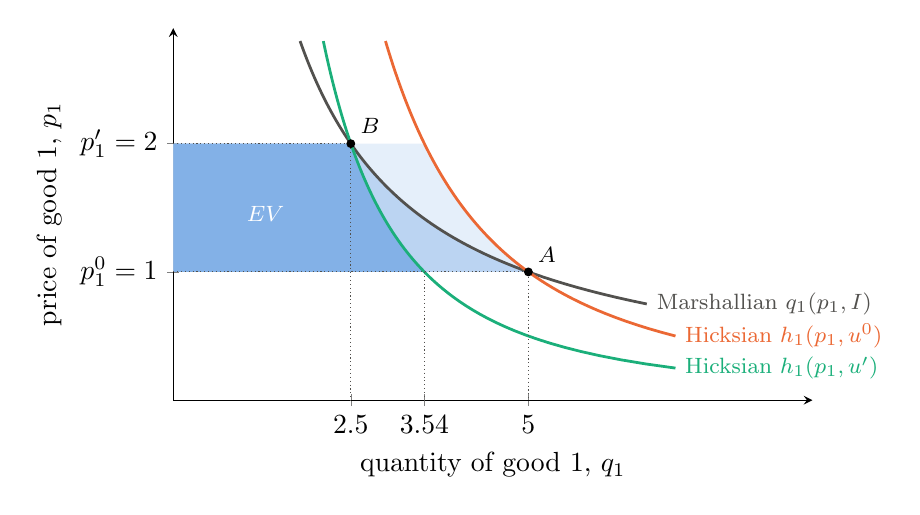
\begin{tikzpicture}
\begin{axis}[
  width=0.8\textwidth, height=0.52\textwidth,
  axis lines=left, xmin=0, xmax=9, ymin=0, ymax=2.9,
  xlabel={quantity of good 1, $q_1$}, ylabel={price of good 1, $p_1$},
  xtick={2.5,3.5355,5}, xticklabels={$2.5$,$3.54$,$5$},
  ytick={1,2}, yticklabels={$p_1^0 = 1$,$p_1' = 2$},
  every axis plot/.append style={line width=1pt},
  clip=false]
\addplot[draw=none, fill=c05p1blue!12, domain=1:2, samples=60, variable=\t]
  ({5/sqrt(\t)},{\t}) -- (axis cs:0,2) -- (axis cs:0,1) -- cycle;
\addplot[draw=none, fill=c05p1blue!32, domain=1:2, samples=60, variable=\t]
  ({5/\t},{\t}) -- (axis cs:0,2) -- (axis cs:0,1) -- cycle;
\addplot[draw=none, fill=c05p1blue!58, domain=1:2, samples=60, variable=\t]
  ({3.5355/sqrt(\t)},{\t}) -- (axis cs:0,2) -- (axis cs:0,1) -- cycle;
\addplot[c05p1gray, domain=0.75:2.8, samples=80, variable=\t] ({5/\t},{\t});
\addplot[c05p1orange, domain=0.5:2.8, samples=80, variable=\t] ({5/sqrt(\t)},{\t});
\addplot[c05p1aqua, domain=0.25:2.8, samples=80, variable=\t] ({3.5355/sqrt(\t)},{\t});
\node[anchor=west, font=\footnotesize, text=c05p1gray] at (axis cs:6.67,0.75) {Marshallian $q_1(p_1, I)$};
\node[anchor=west, font=\footnotesize, text=c05p1orange] at (axis cs:7.07,0.5) {Hicksian $h_1(p_1, u^0)$};
\node[anchor=west, font=\footnotesize, text=c05p1aqua] at (axis cs:7.07,0.25) {Hicksian $h_1(p_1, u')$};
\draw[densely dotted, c05p1gray] (axis cs:0,1) -- (axis cs:5,1) -- (axis cs:5,0);
\draw[densely dotted, c05p1gray] (axis cs:0,2) -- (axis cs:2.5,2) -- (axis cs:2.5,0);
\draw[densely dotted, c05p1gray] (axis cs:3.5355,1) -- (axis cs:3.5355,0);
\fill (axis cs:5,1) circle (1.6pt) node[above right, font=\footnotesize] {$A$};
\fill (axis cs:2.5,2) circle (1.6pt) node[above right, font=\footnotesize] {$B$};
\node[font=\footnotesize, text=white] at (axis cs:1.3,1.45) {$EV$};
\end{axis}
\end{tikzpicture}
\caption{Compensating variation, equivalent variation and Marshallian surplus for a rise in $p_1$ from 1 to 2
(\cref{ex:05-cobb-douglas}: $U = q_1^{\frac{1}{2}}q_2^{\frac{1}{2}}$, $p_2 = 1$, $I = 10$). The consumer
moves from $A$ to $B$ along the Marshallian demand. The Hicksian demand at the initial utility $u^0$ passes
through $A$, and the Hicksian demand at the final utility $u'$ passes through $B$. The darkest region is the
$EV$ (2.93). Adding the middle band gives the Marshallian surplus loss (3.47). Adding the lightest band gives
the $CV$ (4.14).}\label{fig:05-cv-area}
\end{figure}

\subsection{Flexible functional forms}\label{sec:05-flexible}

An empirical demand system must take a parametric form. We want a form general enough not to prejudge the
answers, yet tied to preferences so that it satisfies the restrictions above. The concept that formalizes
``general enough'' is flexibility.

\begin{definition}[Flexible functional form]\label{def:05-flexible}
A parametric expenditure function $e(p, u; \theta)$ is a \emph{flexible functional form} if it can match
any expenditure function to second order at any point \citep{Diewert1974}. Formally, let $(p^0, u^0)$ be any
point and let $\tilde e$ be any twice continuously differentiable expenditure function with the properties of
\cref{prop:05-e-properties}. Then there is a parameter value $\theta$ such that $e$ and $\tilde e$ have the
same value and the same first and second partial derivatives with respect to $(p, u)$ at $(p^0, u^0)$.
\end{definition}

A flexible expenditure function is a second-order approximation to any expenditure function at a point. By
Shephard's lemma its first price derivatives are the Hicksian demands, and its second price derivatives are
the Slutsky terms. The cross derivatives in $p$ and $u$ determine the income effects, because
$\frac{\partial h_i}{\partial u} = \frac{\partial q_i}{\partial I}\frac{\partial e}{\partial u}$. A flexible
expenditure function therefore generates demands whose levels and first derivatives in prices and income can
match those of any demand system at a point. In this sense it is a first-order approximation to demand.

The search for such forms has a long history, which \citet[p.~312]{DeatonMuellbauer1980a} summarize. The
\emph{linear expenditure system} of \citet{Stone1954} was the first system estimated from an explicit utility
function. Its additive utility function leaves only $2J - 1$ free parameters, too few for flexibility, and it
rules out inferior goods and Hicksian complements. The \emph{Rotterdam model} of \citet{Theil1965} and
\citet{Barten1969} approximates the demand functions themselves in differential form, with constant
coefficients on which the restrictions of theory are linear. The \emph{translog model} of
\citet{ChristensenJorgensonLau1975} takes a second-order approximation to the indirect utility function,
$\ln v = \alpha_0 + \sum_i\alpha_i\ln\frac{p_i}{I} + \frac{1}{2}\sum_i\sum_j b_{ij}\ln\frac{p_i}{I}\ln\frac{p_j}{I}$.
By Roy's identity its shares are ratios of linear functions of the log normalized prices, which makes
estimation nonlinear. The AIDS was designed to combine the virtues of these models. It starts from a class
of preferences that permits aggregation over consumers, and it yields shares that are nearly linear in the
parameters.

\section{The Almost Ideal Demand System}\label{sec:05-aids}

\citet{DeatonMuellbauer1980a} derive the AIDS from a specific expenditure function. We follow their
derivation step by step, then establish the restrictions, the elasticities, the flexibility of the system and
its Engel curves, and we close with its limits.

\subsection{The PIGLOG class}\label{sec:05-piglog}

\begin{definition}[PIGLOG preferences]\label{def:05-piglog}
Preferences belong to the \emph{price-independent generalized logarithmic} (PIGLOG) class if the expenditure
function can be written as
\begin{equation}\label{eq:05-piglog}
\ln e(p, u) = (1 - u)\ln a(p) + u\ln b(p),
\end{equation}
where $a(p)$ and $b(p)$ are positive, linearly homogeneous and concave functions of prices.
\end{definition}

Equation \eqref{eq:05-piglog} is equation (1) of \citet[p.~313]{DeatonMuellbauer1980a}, who write the
expenditure function as $c(u, p)$. With some exceptions that they discuss in their appendix, utility lies
between $0$ and $1$. At $u = 0$ expenditure equals $a(p)$, and at $u = 1$ it equals $b(p)$. The two
functions can therefore be regarded as the costs of \emph{subsistence} and of \emph{bliss}
\citep[p.~313]{DeatonMuellbauer1980a}. The class is due to \citet{Muellbauer1975,Muellbauer1976}, who showed
that these preferences permit aggregation over consumers. Market demands can then be represented as if they
were the decisions of one rational representative consumer, with a representative budget level that does not
depend on prices. \Cref{sec:05-aggregation} develops this property.

Two consequences of \eqref{eq:05-piglog} are useful at once. First, the expenditure function equals
$e = a(p)^{1-u}b(p)^u$, a weighted geometric mean of $a$ and $b$. The geometric mean is concave and
increasing in its arguments, so $e$ is concave in $p$ whenever $a$ and $b$ are concave and $0 \leq u \leq 1$.
\citet[p.~324]{DeatonMuellbauer1980a} note that this condition is sufficient for concavity but by no
means necessary. Second, Shephard's lemma in share form gives
\begin{equation}\label{eq:05-piglog-weights}
w_i = (1 - u)\frac{\partial\ln a(p)}{\partial\ln p_i} + u\frac{\partial\ln b(p)}{\partial\ln p_i} .
\end{equation}
Budget shares are weighted averages of the subsistence shares and the bliss shares, with weights given by
utility \citep[p.~324]{DeatonMuellbauer1980a}. Luxuries are the goods whose bliss share exceeds their
subsistence share. Inverting $\ln I = \ln a + u(\ln b - \ln a)$ gives
$u = \frac{\ln I - \ln a(p)}{\ln b(p) - \ln a(p)}$. Substituting into \eqref{eq:05-piglog-weights} shows that
every PIGLOG share is linear in $\ln I$, with intercept and slope that depend on prices:
\begin{equation}\label{eq:05-piglog-share}
w_i = \frac{\partial\ln a(p)}{\partial\ln p_i} + \frac{\partial\ln\frac{b(p)}{a(p)}}{\partial\ln p_i}\cdot
\frac{\ln I - \ln a(p)}{\ln\frac{b(p)}{a(p)}} .
\end{equation}

\subsection{The AIDS cost function}\label{sec:05-aids-cost}

\citet[p.~313]{DeatonMuellbauer1980a} choose specific forms for $a(p)$ and $b(p)$:
\begin{align}
\ln a(p) &= \alpha_0 + \sum_k\alpha_k\ln p_k + \frac{1}{2}\sum_k\sum_j\gamma^*_{kj}\ln p_k\ln p_j,
  \label{eq:05-aids-a}\\
\ln b(p) &= \ln a(p) + \beta_0\prod_k p_k^{\beta_k}. \label{eq:05-aids-b}
\end{align}
Substituting into \eqref{eq:05-piglog} gives the \emph{AIDS cost function}
\begin{equation}\label{eq:05-aids-cost}
\ln e(p, u) = \alpha_0 + \sum_k\alpha_k\ln p_k + \frac{1}{2}\sum_k\sum_j\gamma^*_{kj}\ln p_k\ln p_j
+ u\beta_0\prod_k p_k^{\beta_k},
\end{equation}
where $\alpha_0$, $\alpha_k$, $\beta_0$, $\beta_k$ and $\gamma^*_{kj}$ are parameters. The subsistence cost
$\ln a(p)$ is a translog function of prices, and the gap between bliss and subsistence, $\ln b - \ln a$, is a
Cobb-Douglas function of prices. According to \citet[p.~313]{DeatonMuellbauer1980a}, the choice is governed
partly by the need for flexibility, and mainly by the desirable properties of the demand functions it
generates. At unit prices and $u = 0$ expenditure is $e^{\alpha_0}$, so $e^{\alpha_0}$ is the outlay needed for
subsistence when all prices equal one.

\begin{proposition}[Homogeneity of the AIDS cost function]\label{prop:05-aids-homog}
Let $\gamma_{kj} = \frac{1}{2}(\gamma^*_{kj} + \gamma^*_{jk})$. The function \eqref{eq:05-aids-cost} is
homogeneous of degree one in $p$ for all $u$ if and only if
\begin{equation}\label{eq:05-aids-homog}
\sum_k\alpha_k = 1, \qquad \sum_j\gamma_{kj} = 0 \ \text{ for every } k, \qquad \sum_k\beta_k = 0 .
\end{equation}
In particular, the conditions $\sum_j\gamma^*_{kj} = \sum_k\gamma^*_{kj} = 0$ stated by
\citet[p.~313]{DeatonMuellbauer1980a}, together with $\sum_k\alpha_k = 1$ and $\sum_k\beta_k = 0$, are
sufficient.
\end{proposition}

\begin{proof}
The quadratic form depends on $\gamma^*$ only through its symmetric part, because for any vector $x$
\begin{equation*}
\sum_k\sum_j\gamma^*_{kj}x_kx_j = \sum_k\sum_j\gamma_{kj}x_kx_j .
\end{equation*}
Write
$\ell = \ln\lambda$ and $R_k = \sum_j\gamma_{kj}$. Replace $\ln p_k$ by $\ln p_k + \ell$ in
\eqref{eq:05-aids-cost} and subtract $\ln e(p, u) + \ell$. The linear part contributes
$\big(\sum_k\alpha_k - 1\big)\ell$. The quadratic part contributes
\begin{equation*}
\frac{1}{2}\sum_k\sum_j\gamma_{kj}\big[(\ln p_k + \ell)(\ln p_j + \ell) - \ln p_k\ln p_j\big]
= \ell\sum_k R_k\ln p_k + \frac{1}{2}\ell^2\sum_k R_k ,
\end{equation*}
where we used the symmetry of $\gamma$ to combine the two cross terms. The last term contributes
$u\beta_0\prod_k p_k^{\beta_k}\big(\lambda^{\sum_k\beta_k} - 1\big)$. Under \eqref{eq:05-aids-homog} every
contribution vanishes, which proves sufficiency. For necessity, the total must vanish for all $\lambda$, $p$
and $u$. At $u = 0$ and unit prices it equals $\big(\sum_k\alpha_k - 1\big)\ell + \frac{1}{2}\ell^2\sum_kR_k$,
so $\sum_k\alpha_k = 1$ and $\sum_kR_k = 0$. At $u = 0$ and arbitrary prices it then equals
$\ell\sum_kR_k\ln p_k$, so every $R_k = 0$. At $u > 0$ the remaining term forces
$\lambda^{\sum_k\beta_k} = 1$ for all $\lambda$, that is, $\sum_k\beta_k = 0$. The stated conditions on
$\gamma^*$ imply $R_k = \frac{1}{2}\big(\sum_j\gamma^*_{kj} + \sum_j\gamma^*_{jk}\big) = 0$.
\end{proof}

\begin{remark}[Two normalizations]\label{rem:05-aids-normalizations}
The expenditure function depends on $u$ and $\beta_0$ only through their product $u\beta_0$. Replacing $u$ by
$\frac{u}{c}$ and $\beta_0$ by $c\beta_0$ for any $c > 0$ changes nothing observable, because it only
rescales utility. Since utility is ordinal, we may set $\beta_0 = 1$, and we do so in numerical work. The
expenditure function increases in $u$ only if $\beta_0 > 0$. The second normalization concerns curvature in
utility. Because $\ln e$ is linear in $u$, the AIDS sets $\frac{\partial^2\ln e}{\partial u^2} = 0$
everywhere. \citet[p.~313]{DeatonMuellbauer1980a} point out that this costs no generality, because an
ordinal normalization of utility can always set this derivative to zero at a point.
\end{remark}

A parameter count shows that the AIDS cost function has just enough parameters to be flexible. Consider an
arbitrary expenditure function and a point $(p^0, u^0)$. Its value, its $J$ price derivatives and its
derivative in $u$ make $J + 2$ numbers. Its second derivatives add $\frac{J(J+1)}{2}$ distinct price terms,
$J$ cross terms in $p$ and $u$, and one term in $u$, for a total of $\frac{J(J+1)}{2} + 2J + 3$. Homogeneity of
degree one imposes Euler's equation on the value, on the first price derivatives and on the derivative in
$u$, which removes $J + 2$ of them. That leaves $\frac{(J+1)(J+2)}{2}$ free numbers. The AIDS has
$\alpha_0$, $J - 1$ free $\alpha_k$, $\frac{J(J-1)}{2}$ free $\gamma_{kj}$, $J - 1$ free $\beta_k$ and
$\beta_0$, which is $\frac{J(J+3)}{2}$ parameters. The difference is exactly one, the second derivative in
$u$, which the ordinal normalization of \cref{rem:05-aids-normalizations} absorbs. A count is necessary but
not sufficient for flexibility. \Cref{prop:05-flexible} proves the corresponding property for demands by
construction.

\subsection{Deriving the share equations}\label{sec:05-aids-shares}

We derive the budget shares in six steps.

\casehead{Step 1} Shephard's lemma in share form gives the shares. By \eqref{eq:05-shephard-share}, the budget share of good $i$
is the derivative of \eqref{eq:05-aids-cost} with respect to $\ln p_i$
\citep[eq.~5]{DeatonMuellbauer1980a}:
\begin{equation*}
w_i = \frac{\partial\ln e(p, u)}{\partial\ln p_i}.
\end{equation*}

\casehead{Step 2} We differentiate the translog part. The linear term contributes $\alpha_i$. In the quadratic term, $\ln p_i$
appears once as $\ln p_k$ (when $k = i$) and once as $\ln p_j$ (when $j = i$):
\begin{equation*}
\frac{\partial}{\partial\ln p_i}\Big[\frac{1}{2}\sum_k\sum_j\gamma^*_{kj}\ln p_k\ln p_j\Big]
= \frac{1}{2}\sum_j\gamma^*_{ij}\ln p_j + \frac{1}{2}\sum_k\gamma^*_{ki}\ln p_k
= \sum_j\gamma_{ij}\ln p_j ,
\end{equation*}
where
\begin{equation}\label{eq:05-gamma-sym}
\gamma_{ij} = \frac{1}{2}\big(\gamma^*_{ij} + \gamma^*_{ji}\big)
\end{equation}
is equation (7) of \citet{DeatonMuellbauer1980a}. The coefficients $\gamma_{ij}$ that enter the share
equations are symmetric by construction when the system is derived from the cost function.

\casehead{Step 3} We differentiate the Cobb-Douglas part. Write the product as an exponential and differentiate:
\begin{equation*}
\frac{\partial}{\partial\ln p_i}\prod_k p_k^{\beta_k} = \frac{\partial}{\partial\ln p_i}
\exp\Big(\sum_k\beta_k\ln p_k\Big) = \beta_i\prod_k p_k^{\beta_k}.
\end{equation*}

\casehead{Step 4} Collecting the three pieces gives the shares as functions of prices and
utility \citep[eq.~6]{DeatonMuellbauer1980a}:
\begin{equation}\label{eq:05-aids-hicks-share}
w_i(p, u) = \alpha_i + \sum_j\gamma_{ij}\ln p_j + \beta_iu\beta_0\prod_k p_k^{\beta_k} .
\end{equation}

\casehead{Step 5} We now solve for indirect utility. Define the \emph{translog price index}
\begin{equation}\label{eq:05-translog}
\ln\mathbf{P}(p) = \alpha_0 + \sum_k\alpha_k\ln p_k + \frac{1}{2}\sum_k\sum_j\gamma_{kj}\ln p_k\ln p_j ,
\end{equation}
which is equation (9) of \citet{DeatonMuellbauer1980a}. By the first step of the proof of
\cref{prop:05-aids-homog}, $\ln\mathbf{P}(p) = \ln a(p)$, so the price index is the subsistence cost. Write
\begin{equation}\label{eq:05-aids-B}
B(p) = \beta_0\prod_k p_k^{\beta_k} = \ln b(p) - \ln a(p)
\end{equation}
for the Cobb-Douglas part of the cost function. The cost function becomes
$\ln e(p, u) = \ln\mathbf{P}(p) + u\,B(p)$. A utility-maximizing consumer spends $e(p, u) = I$. Solving for
$u$ gives the indirect utility function
\begin{equation}\label{eq:05-aids-v}
v(p, I) = \frac{\ln I - \ln\mathbf{P}(p)}{B(p)} .
\end{equation}

\casehead{Step 6} We obtain the Marshallian shares. At $u = v(p, I)$, the last term of
\eqref{eq:05-aids-hicks-share} equals $\beta_iuB(p) = \beta_i\big(\ln I - \ln\mathbf{P}\big)$. The AIDS demand functions in budget share form are therefore
\begin{equation}\label{eq:05-aids-share}
w_i = \alpha_i + \sum_{j=1}^J\gamma_{ij}\ln p_j + \beta_i\ln\frac{I}{\mathbf{P}} ,
\qquad i = 1, \dots, J,
\end{equation}
which is equation (8) of \citet{DeatonMuellbauer1980a}.

Roy's identity gives the same result from \eqref{eq:05-aids-v}, which is a useful check. By Step 3,
$\frac{\partial B}{\partial\ln p_i} = \beta_iB$. Then $\frac{\partial v}{\partial\ln I} = \frac{1}{B}$ and
\begin{equation*}
\frac{\partial v}{\partial\ln p_i} = -\frac{1}{B}\frac{\partial\ln\mathbf{P}}{\partial\ln p_i}
- \frac{\ln I - \ln\mathbf{P}}{B}\beta_i .
\end{equation*}
The share form of \eqref{eq:05-roy} gives
$w_i = \frac{\partial\ln\mathbf{P}}{\partial\ln p_i} + \beta_i\ln\frac{I}{\mathbf{P}}$. Step 2 applied to
\eqref{eq:05-translog} gives $\frac{\partial\ln\mathbf{P}}{\partial\ln p_i} = \alpha_i + \sum_j\gamma_{ij}\ln
p_j$, which reproduces \eqref{eq:05-aids-share}.

The parameters have simple interpretations \citep[p.~314]{DeatonMuellbauer1980a}. When relative prices and
real expenditure $\frac{I}{\mathbf{P}}$ do not change, the budget shares are constant. This is the natural
starting point for predictions with the model. Changes in relative prices work through the $\gamma_{ij}$.
Each $\gamma_{ij}$ is 100 times the change in the budget share of good $i$ caused by a one percent rise in
$p_j$ with $\frac{I}{\mathbf{P}}$ held constant. The factor 100 appears because such a rise increases
$\ln p_j$ by about $0.01$.
Changes in real expenditure work through the $\beta_i$, which sum to zero. They are positive for luxuries and
negative for necessities, as \eqref{eq:05-eta} below confirms. Real expenditure is measured relative to the
subsistence cost $\mathbf{P}(p) = a(p)$. The price index depends on the parameters $\alpha_0$, $\alpha_k$ and
$\gamma_{kj}$, which makes the system nonlinear in its parameters. \Cref{sec:05-estimation} discusses how to
estimate it, including the common approximation of $\mathbf{P}$ by a price index computed from data.

\begin{remark}[From Engel curves to the AIDS]\label{rem:05-working-leser}
\citet[\S 3.4, pp.~75--77]{DeatonMuellbauer1980b} reach the AIDS from the data side. Budget studies
support the \emph{Working-Leser} Engel curve, in which the budget share is linear in the log budget, $w_i
= \tilde\alpha_i + \tilde\beta_i\ln I$ at fixed prices (their eq.~4.1, \citealp{Working1943,Leser1963}). To
use it on time series, the coefficients must become functions of prices in a way consistent with
preferences. Any expenditure function of the form
\begin{equation*}
  \ln e(p, u) = A(p) + u\,B(p)
\end{equation*}
does this (their eq.~4.2). Write $A_i = \frac{\partial A}{\partial\ln p_i}$ and $B_i = \frac{\partial
B}{\partial\ln p_i}$. Shephard's lemma in share form gives $w_i = A_i(p) + u\,B_i(p)$. Inverting $\ln I =
A(p) + uB(p)$ gives $u = \frac{\ln I - A(p)}{B(p)}$. Substituting,
\begin{equation*}
  w_i = \Bigl[A_i(p) - \frac{B_i(p)}{B(p)}A(p)\Bigr] + \frac{B_i(p)}{B(p)}\ln I ,
\end{equation*}
which has the Working-Leser form at every price vector. The AIDS chooses $A(p)$ translog and $B(p) =
\beta_0\prod_k p_k^{\beta_k}$, as in their eqs.~(4.3)--(4.4). Then $\frac{B_i}{B} = \beta_i$ is constant,
$A_i = \alpha_i + \sum_j\gamma_{ij}\ln p_j$, and the display becomes \eqref{eq:05-aids-share}. The book's
$A(p)$ is the article's $\ln a(p)$, and its $B(p)$ is the article's $\ln b(p) - \ln a(p)$, which is
\eqref{eq:05-aids-B}. The two derivations therefore describe the same model. The book also states the
negativity condition with a matrix $C$, its eq.~(4.12), which is our $K$ of \eqref{eq:05-K}. It stresses
that the matrix $[\gamma_{ij}]$ itself need not be negative semidefinite (p.~76).
\end{remark}

\subsection{Restrictions from consumer theory}\label{sec:05-aids-restrictions}

Suppose we take the share equations \eqref{eq:05-aids-share} with the index \eqref{eq:05-translog} as a
maintained hypothesis, with unrestricted coefficients $\gamma_{ij}$, as
\citet[p.~316]{DeatonMuellbauer1980a} do. The next proposition states which linear restrictions make the
system consistent with demand theory.

\begin{proposition}[Adding up, homogeneity and symmetry]\label{prop:05-restrictions}
Consider \eqref{eq:05-aids-share} and \eqref{eq:05-translog}.
\begin{enumerate}[label=(\roman*)]
\item The shares sum to one at all $(p, I)$ if and only if
  \begin{equation}\label{eq:05-adding-up}
  \sum_i\alpha_i = 1, \qquad \sum_i\gamma_{ij} = 0 \ \text{ for every } j, \qquad \sum_i\beta_i = 0 .
  \end{equation}
\item Given \eqref{eq:05-adding-up}, demands are homogeneous of degree zero in $(p, I)$ if and only if
  \begin{equation}\label{eq:05-homogeneity}
  \sum_j\gamma_{ij} = 0 \ \text{ for every } i .
  \end{equation}
\item Given \eqref{eq:05-adding-up} and \eqref{eq:05-homogeneity}, the Slutsky matrix is symmetric at all
  $(p, I)$ if and only if
  \begin{equation}\label{eq:05-symmetry}
  \gamma_{ij} = \gamma_{ji} \ \text{ for all } i, j .
  \end{equation}
\end{enumerate}
\end{proposition}

\begin{proof}
(i) Sum \eqref{eq:05-aids-share} over $i$:
\begin{equation*}
\sum_iw_i = \sum_i\alpha_i + \sum_j\Big(\sum_i\gamma_{ij}\Big)\ln p_j + \Big(\sum_i\beta_i\Big)\ln\frac{I}{\mathbf{P}} .
\end{equation*}
Given $p$, the term $\ln I$ varies freely, so the sum equals one for all $I$ only if $\sum_i\beta_i = 0$.
Then $\sum_j\big(\sum_i\gamma_{ij}\big)\ln p_j = 1 - \sum_i\alpha_i$ for all log prices, which requires every
coefficient to vanish and the constant to be zero. The converse is immediate.

(ii) Write $\ell = \ln\lambda$ and $R_i = \sum_j\gamma_{ij}$. Because \eqref{eq:05-adding-up} makes the
column sums of $\gamma$ zero and $\sum_k\alpha_k = 1$, the computation in the proof of
\cref{prop:05-aids-homog} gives
$\ln\mathbf{P}(\lambda p) = \ln\mathbf{P}(p) + \ell + \frac{1}{2}\ell\sum_kR_k\ln p_k + \frac{1}{2}\ell^2\sum_kR_k$.
Hence
\begin{equation*}
w_i(\lambda p, \lambda I) - w_i(p, I) = \ell R_i - \beta_i\Big[\frac{1}{2}\ell\sum_kR_k\ln p_k +
\frac{1}{2}\ell^2\sum_kR_k\Big].
\end{equation*}
If every $R_k = 0$, the difference vanishes. Conversely, at unit prices the difference is
$\ell R_i - \frac{1}{2}\beta_i\ell^2\sum_kR_k$, and it vanishes for all $\lambda$ only if $R_i = 0$.

(iii) Let $\gamma^s_{jk} = \frac{1}{2}(\gamma_{jk} + \gamma_{kj})$ and $r = \ln\frac{I}{\mathbf{P}}$. Then
$\frac{\partial w_i}{\partial\ln I} = \beta_i$, $\frac{\partial\ln\mathbf{P}}{\partial\ln p_j} = \alpha_j +
\sum_k\gamma^s_{jk}\ln p_k$, and
$\frac{\partial w_i}{\partial\ln p_j} = \gamma_{ij} - \beta_i\frac{\partial\ln\mathbf{P}}{\partial\ln p_j}$.
Using $w_j = \alpha_j + \sum_k\gamma_{jk}\ln p_k + \beta_jr$, the first two terms of \eqref{eq:05-K-general}
are
\begin{equation*}
\frac{\partial w_i}{\partial\ln p_j} + w_j\frac{\partial w_i}{\partial\ln I}
= \gamma_{ij} + \beta_i\beta_jr + \beta_i\sum_k\big(\gamma_{jk} - \gamma^s_{jk}\big)\ln p_k .
\end{equation*}
The remaining terms of \eqref{eq:05-K-general}, $w_iw_j - \indic(i=j)w_i$, are symmetric in $(i, j)$. Under
\eqref{eq:05-symmetry} the last sum vanishes and $k_{ij} = \gamma_{ij} + \beta_i\beta_jr + w_iw_j -
\indic(i=j)w_i$ is symmetric, so $S_{ij} = \frac{I\,k_{ij}}{p_ip_j}$ is symmetric. Conversely, at unit prices the
expression reduces to $\gamma_{ij} + \beta_i\beta_jr$, which is symmetric only if $\gamma_{ij} = \gamma_{ji}$.
\end{proof}

These are equations (10) to (12) of \citet[p.~314]{DeatonMuellbauer1980a}. All three sets are linear in the
parameters and do not involve the data, so they can be imposed globally by standard methods. They differ in
how they can be tested \citep[p.~316]{DeatonMuellbauer1980a}. Adding up cannot be tested on share data,
because observed shares add up to one by construction and the estimated parameters satisfy
\eqref{eq:05-adding-up} automatically. Homogeneity involves the parameters of a single equation and can be
tested equation by equation. Symmetry links the parameters of two equations and can only be tested in a
system. \Cref{sec:05-testing} carries out these tests.

\subsection{Negativity}\label{sec:05-negativity}

Concavity of the expenditure function is the fourth restriction, and it is of a different kind.

\begin{proposition}[Negativity of the AIDS]\label{prop:05-negativity}
Under \eqref{eq:05-adding-up}, \eqref{eq:05-homogeneity} and \eqref{eq:05-symmetry}, the Slutsky terms of the
AIDS satisfy
\begin{equation}\label{eq:05-hicks-deriv}
\frac{\partial h_i(p, u)}{\partial p_j} = \frac{e(p, u)}{p_ip_j}\Big[\frac{\partial w_i(p,u)}{\partial\ln p_j}
+ w_iw_j - \indic(i=j)w_i\Big],
\end{equation}
where $w_i(p, u)$ is the Hicksian share \eqref{eq:05-aids-hicks-share}. The matrix $K = [k_{ij}]$ with
$k_{ij} = \frac{p_ip_jS_{ij}}{I}$ equals
\begin{equation}\label{eq:05-K}
k_{ij} = \gamma_{ij} + \beta_i\beta_j\ln\frac{I}{\mathbf{P}} - \indic(i=j)w_i + w_iw_j ,
\end{equation}
and its eigenvalues have the same signs as those of $S$. The AIDS satisfies negativity at $(p, I)$ if and
only if $K$ is negative semidefinite there.
\end{proposition}

\begin{proof}
By Shephard's lemma and \eqref{eq:05-shephard-share}, $h_i = \frac{w_i(p,u)e(p,u)}{p_i}$. Differentiate with
respect to $p_j$ by the product rule:
\begin{equation*}
\frac{\partial h_i}{\partial p_j} = \frac{e}{p_i}\frac{\partial w_i}{\partial p_j} + \frac{w_i}{p_i}
\frac{\partial e}{\partial p_j} - \indic(i=j)\frac{w_ie}{p_i^2} .
\end{equation*}
Substitute $\frac{\partial w_i}{\partial p_j} = \frac{1}{p_j}\frac{\partial w_i}{\partial\ln p_j}$ and
$\frac{\partial e}{\partial p_j} = h_j = \frac{w_je}{p_j}$, and factor out $\frac{e}{p_ip_j}$ to obtain
\eqref{eq:05-hicks-deriv}. For the AIDS, differentiating \eqref{eq:05-aids-hicks-share} and using Step 3 gives
\begin{equation*}
\frac{\partial w_i(p, u)}{\partial\ln p_j} = \gamma_{ij} + \beta_i\beta_ju\beta_0\prod_kp_k^{\beta_k}
= \gamma_{ij} + \beta_i\beta_j\ln\frac{I}{\mathbf{P}} ,
\end{equation*}
where the second equality evaluates at $u = v(p, I)$. Multiplying \eqref{eq:05-hicks-deriv} by
$\frac{p_ip_j}{I}$ with $e = I$ gives \eqref{eq:05-K}. Finally, $K = \frac{1}{I}DSD$ with
$D = \diag(p_1, \dots, p_J)$ nonsingular. By Sylvester's law of inertia, congruent symmetric matrices have
the same numbers of positive, negative and zero eigenvalues.
\end{proof}

Equation \eqref{eq:05-K} is equation (14) of \citet[p.~316]{DeatonMuellbauer1980a}. It agrees with the
general formula \eqref{eq:05-K-general}, as the proof of \cref{prop:05-restrictions} showed. Three features
matter in practice. First, the rows of $K$ sum to zero:
$\sum_jk_{ij} = \sum_j\gamma_{ij} + \beta_i\ln\frac{I}{\mathbf{P}}\sum_j\beta_j - w_i + w_i\sum_jw_j = 0$. This is the share-form
counterpart of $Sp = 0$. One eigenvalue of $K$ is therefore identically zero, and negativity requires the
other $J - 1$ eigenvalues to be nonpositive. Second, $K$ depends on the data point through the shares and
through $\ln\frac{I}{\mathbf{P}}$. As with other flexible forms, no restriction on the parameters alone can
guarantee negativity \citep[p.~316]{DeatonMuellbauer1980a}. Negativity can be checked observation by
observation by computing the eigenvalues of $K$ at the estimates. It can also be imposed at a single point. We
write $K$ at that point as $-LL^\T$, with $L$ lower triangular, and estimate the elements of $L$ in place of
the $\gamma_{ij}$ \citep{Lau1978,Moschini1999}. Third, part (f) of \cref{prop:05-elast-identities} gives
$\varepsilon^h_{ij} = \frac{k_{ij}}{w_i}$, so that for $i \neq j$
\begin{equation}\label{eq:05-gamma-sign}
\varepsilon^h_{ij} = \frac{\gamma_{ij} + \beta_i\beta_j\ln\frac{I}{\mathbf{P}}}{w_i} + w_j .
\end{equation}
When $\beta_i\beta_j\ln\frac{I}{\mathbf{P}} + w_iw_j$ is small relative to $\gamma_{ij}$, the coefficient
$\gamma_{ij}$ has the sign of the compensated cross-price elasticity. This is the approximation that
\citet[p.~315]{DeatonMuellbauer1980a} invoke when they suggest using prior beliefs about substitutes and
complements to restrict individual $\gamma_{ij}$.

\subsection{Elasticities}\label{sec:05-aids-elasticities}

The elasticities follow from three derivatives of the Marshallian shares. Throughout, write
$r = \ln\frac{I}{\mathbf{P}}$ and impose \eqref{eq:05-adding-up}, \eqref{eq:05-homogeneity} and
\eqref{eq:05-symmetry}. The derivative with respect to log income is
\begin{equation}\label{eq:05-dw-dI}
\frac{\partial w_i}{\partial\ln I} = \beta_i .
\end{equation}
Differentiating the translog index as in Step 2 and using the share equation for good $j$ gives
\begin{equation}\label{eq:05-dlnP}
\frac{\partial\ln\mathbf{P}}{\partial\ln p_j} = \alpha_j + \sum_k\gamma_{jk}\ln p_k = w_j - \beta_jr .
\end{equation}
The derivative with respect to a log price therefore has two equivalent forms:
\begin{equation}\label{eq:05-dw-dp}
\frac{\partial w_i}{\partial\ln p_j} = \gamma_{ij} - \beta_i\Big(\alpha_j + \sum_k\gamma_{jk}\ln p_k\Big)
= \gamma_{ij} - \beta_i\big(w_j - \beta_jr\big).
\end{equation}

To convert share derivatives into elasticities, write $q_i = \frac{w_iI}{p_i}$, so that
$\ln q_i = \ln w_i + \ln I - \ln p_i$. Differentiating with respect to $\ln I$ gives the expenditure
elasticity
\begin{equation}\label{eq:05-eta}
\eta_i = 1 + \frac{1}{w_i}\frac{\partial w_i}{\partial\ln I} = 1 + \frac{\beta_i}{w_i} .
\end{equation}
A good is a luxury ($\eta_i > 1$) if and only if $\beta_i > 0$, and a necessity if and only if
$\beta_i < 0$. Differentiating with respect to $\ln p_j$ gives the Marshallian price elasticity
\begin{equation}\label{eq:05-elast-marshall}
\varepsilon_{ij} = -\indic(i=j) + \frac{1}{w_i}\frac{\partial w_i}{\partial\ln p_j}
= -\indic(i=j) + \frac{\gamma_{ij} - \beta_i\big(w_j - \beta_j\ln\frac{I}{\mathbf{P}}\big)}{w_i} .
\end{equation}
The Slutsky equation of \cref{prop:05-elast-identities}(a) gives the Hicksian elasticity. Adding
$\eta_iw_j = w_j + \frac{\beta_iw_j}{w_i}$ to \eqref{eq:05-elast-marshall}, the terms in $\beta_iw_j$ cancel:
\begin{equation}\label{eq:05-elast-hicks}
\varepsilon^h_{ij} = \varepsilon_{ij} + \eta_iw_j
= -\indic(i=j) + w_j + \frac{\gamma_{ij} + \beta_i\beta_j\ln\frac{I}{\mathbf{P}}}{w_i} .
\end{equation}
This agrees with $\varepsilon^h_{ij} = \frac{k_{ij}}{w_i}$ from \eqref{eq:05-K}. Note that
\eqref{eq:05-elast-marshall} uses the derivative of the exact index \eqref{eq:05-dlnP}. Approximating that
derivative by $w_j$, as is common when $\mathbf{P}$ is replaced by a data index, changes the formula. We
return to this point in \cref{sec:05-stone}.

The elasticities satisfy the identities of \cref{prop:05-elast-identities} under the restrictions. Engel
aggregation holds because $\sum_iw_i\eta_i = \sum_iw_i + \sum_i\beta_i = 1$. Cournot aggregation holds
because
\begin{equation*}
\sum_iw_i\varepsilon_{ij} = -w_j + \sum_i\gamma_{ij} - \big(w_j - \beta_jr\big)\sum_i\beta_i = -w_j ,
\end{equation*}
using the adding-up restrictions on $\gamma$ and $\beta$. Homogeneity holds because
\begin{equation*}
\sum_j\varepsilon_{ij} + \eta_i = -1 + \frac{1}{w_i}\Big[\sum_j\gamma_{ij} - \beta_i\sum_j\alpha_j -
\beta_i\sum_k\Big(\sum_j\gamma_{jk}\Big)\ln p_k\Big] + 1 + \frac{\beta_i}{w_i} = 0 ,
\end{equation*}
where $\sum_j\gamma_{ij} = 0$ by homogeneity, and $\sum_j\alpha_j = 1$ and $\sum_j\gamma_{jk} = 0$ by adding
up. Symmetry holds because $w_i\varepsilon^h_{ij} = k_{ij}$ and $K$ is symmetric.

\begin{example}[The running example]\label{ex:05-running}
We use one numerical AIDS throughout the chapter. There are three goods, with $\alpha_0 = 0$,
$\alpha = (0.5, 0.3, 0.2)$, $\beta = (-0.10, 0.04, 0.06)$ and
\begin{equation*}
\Gamma = [\gamma_{ij}] = \begin{pmatrix} -0.20 & 0.12 & 0.08\\ 0.12 & -0.22 & 0.10\\ 0.08 & 0.10 & -0.18
\end{pmatrix}.
\end{equation*}
The parameters satisfy adding up, homogeneity and symmetry, since $\sum_i\alpha_i = 1$,
$\sum_i\beta_i = 0$, and $\Gamma$ is symmetric with zero row and column sums. Evaluate the system at
$p = (1, 1, 1)$ and $\ln I = 1$. All log prices are zero, so $\ln\mathbf{P} = \alpha_0 = 0$ and
$\ln\frac{I}{\mathbf{P}} = 1$. The shares are $w_i = \alpha_i + \beta_i$, that is,
$w = (0.40, 0.34, 0.26)$. Good 1 is a necessity, with $\eta_1 = 1 - \frac{0.10}{0.40} = 0.75$, and goods 2
and 3 are luxuries. For the own-price elasticity of good 1, \eqref{eq:05-elast-marshall} gives
\begin{equation*}
\varepsilon_{11} = -1 + \frac{-0.20 - (-0.10)\big(0.40 - (-0.10)(1)\big)}{0.40} = -1 + \frac{-0.15}{0.40}
= -1.375 ,
\end{equation*}
and the Hicksian elasticity is $\varepsilon^h_{11} = -1.375 + 0.75 \times 0.40 = -1.075$. The diagonal
element of $K$ is $k_{11} = -0.20 + 0.01 - 0.40 + 0.16 = -0.43$, and indeed
$\frac{k_{11}}{w_1} = -1.075$. \Cref{tab:05-running-example} reports the full matrices, computed with the
script \texttt{figures/ch05/src/aids\_example.py}. The identities hold to rounding. For the first column,
Cournot aggregation gives $0.40(-1.375) + 0.34(0.294) + 0.26(0.192) = -0.40 = -w_1$. For the first row,
homogeneity gives $-1.375 + 0.375 + 0.250 + 0.750 = 0$. Symmetry gives
$w_1\varepsilon^h_{12} = 0.40 \times 0.630 = 0.252 = 0.34 \times 0.741 = w_2\varepsilon^h_{21}$. The nonzero
eigenvalues of $K$ are $-0.689$ and $-0.552$, so the cost function is concave at this point.
\end{example}

\begin{table}[htbp]
\centering
\caption{The running example at $p = (1, 1, 1)$ and $\ln I = 1$}\label{tab:05-running-example}
\small
\begin{tabular}{c *{7}{S[table-format=-1.3]}}
\toprule
\multicolumn{8}{l}{\textit{A. Parameters, budget shares and expenditure elasticities} ($\alpha_0 = 0$)} \\
\midrule
Good $i$ & {$\alpha_i$} & {$\beta_i$} & {$\gamma_{i1}$} & {$\gamma_{i2}$} & {$\gamma_{i3}$} & {$w_i$} & {$\eta_i$} \\
\midrule
1 & 0.50 & -0.10 & -0.20 & 0.12 & 0.08 & 0.400 & 0.750 \\
2 & 0.30 & 0.04 & 0.12 & -0.22 & 0.10 & 0.340 & 1.118 \\
3 & 0.20 & 0.06 & 0.08 & 0.10 & -0.18 & 0.260 & 1.231 \\
\bottomrule
\end{tabular}

\medskip
\begin{tabular}{c *{9}{S[table-format=-1.3]}}
\toprule
\multicolumn{10}{l}{\textit{B. Price elasticities and the negativity matrix} (row $i$, price $j$)} \\
\midrule
 & \multicolumn{3}{c}{Marshallian $\varepsilon_{ij}$} & \multicolumn{3}{c}{Hicksian $\varepsilon^h_{ij}$}
 & \multicolumn{3}{c}{$k_{ij}$, equation \eqref{eq:05-K}} \\
\cmidrule(lr){2-4}\cmidrule(lr){5-7}\cmidrule(lr){8-10}
Good $i$ & {$j = 1$} & {$j = 2$} & {$j = 3$} & {$j = 1$} & {$j = 2$} & {$j = 3$} & {$j = 1$} & {$j = 2$}
 & {$j = 3$} \\
\midrule
1 & -1.375 & 0.375 & 0.250 & -1.075 & 0.630 & 0.445 & -0.430 & 0.252 & 0.178 \\
2 & 0.294 & -1.682 & 0.271 & 0.741 & -1.302 & 0.561 & 0.252 & -0.443 & 0.191 \\
3 & 0.192 & 0.315 & -1.738 & 0.685 & 0.734 & -1.418 & 0.178 & 0.191 & -0.369 \\
\midrule
\multicolumn{7}{l}{Eigenvalues of $K$} & -0.689 & -0.552 & 0.000 \\
\bottomrule
\end{tabular}
\par\smallskip
\begin{minipage}{0.92\textwidth}\footnotesize\raggedright
Notes: Elasticities are signed and computed from \eqref{eq:05-eta}, \eqref{eq:05-elast-marshall} and
\eqref{eq:05-elast-hicks}. The script \texttt{figures/ch05/src/aids\_example.py} also checks every analytic
elasticity against numerical derivatives of the demand functions, with a maximum discrepancy below $10^{-9}$.
\end{minipage}
\end{table}

\subsection{Flexibility*}\label{sec:05-aids-flexibility}

\citet[p.~315]{DeatonMuellbauer1980a} claim that the AIDS demand functions are first-order approximations to
any demand system, whether or not that system comes from utility maximization. We make the claim precise and
prove it by construction. A preliminary fact lets us work at unit prices.

\begin{lemma}[Units of measurement]\label{lem:05-units}
Let $\Gamma$ be symmetric, and measure good $k$ in new units, so that $\ln p_k = \ln\tilde p_k + c_k$ for
constants $c_k$. The AIDS in the new prices has the same $\gamma_{ij}$ and $\beta_i$, and the parameters
\begin{equation*}
\tilde\alpha_k = \alpha_k + \sum_j\gamma_{kj}c_j, \qquad
\tilde\alpha_0 = \alpha_0 + \sum_k\alpha_kc_k + \frac{1}{2}\sum_k\sum_j\gamma_{kj}c_kc_j .
\end{equation*}
These parameters satisfy \eqref{eq:05-adding-up}, \eqref{eq:05-homogeneity} and \eqref{eq:05-symmetry}
whenever the original ones do.
\end{lemma}

\begin{proof}
Substitute $\ln p_k = \ln\tilde p_k + c_k$ into \eqref{eq:05-translog} and expand the quadratic term, using
the symmetry of $\Gamma$ to combine the two cross terms:
\begin{equation*}
\ln\mathbf{P} = \Big[\alpha_0 + \sum_k\alpha_kc_k + \frac{1}{2}\sum_k\sum_j\gamma_{kj}c_kc_j\Big]
+ \sum_k\Big(\alpha_k + \sum_j\gamma_{kj}c_j\Big)\ln\tilde p_k
+ \frac{1}{2}\sum_k\sum_j\gamma_{kj}\ln\tilde p_k\ln\tilde p_j .
\end{equation*}
This is the translog index in the new prices with parameters $\tilde\alpha_0$ and $\tilde\alpha_k$. In the
share equation, $\alpha_i + \sum_j\gamma_{ij}\ln p_j = \tilde\alpha_i + \sum_j\gamma_{ij}\ln\tilde p_j$, and
income is unaffected. Hence every share is the same function of the data in either set of units. Finally,
$\sum_k\tilde\alpha_k = \sum_k\alpha_k + \sum_jc_j\sum_k\gamma_{kj} = 1$ under adding up, and $\Gamma$ is
unchanged.
\end{proof}

Fitted shares and elasticities therefore do not depend on the units in which goods are measured. Given any
point $(p^0, I^0)$, we can choose units so that $p^0 = (1, \dots, 1)$. We state the flexibility result at such
a point.

\begin{proposition}[First-order flexibility]\label{prop:05-flexible}
Fix a point $(p^0, I^0)$ with $p^0 = (1, \dots, 1)$. Let $w^0$ be any vector of positive budget shares that sum
to one, let $b_i$ be any numbers with $\sum_ib_i = 0$, and let $c_{ij}$ be any numbers with
$\sum_ic_{ij} = 0$ for every $j$.
\begin{enumerate}[label=(\roman*)]
\item There are AIDS parameters satisfying \eqref{eq:05-adding-up} such that, at $(p^0, I^0)$,
  $w_i = w^0_i$, $\frac{\partial w_i}{\partial\ln I} = b_i$ and $\frac{\partial w_i}{\partial\ln p_j} = c_{ij}$.
\item If in addition $\sum_jc_{ij} + b_i = 0$ for every $i$ (homogeneity) and $c_{ij} + b_iw^0_j$ is
  symmetric in $(i, j)$ (Slutsky symmetry), the parameters also satisfy \eqref{eq:05-homogeneity} and
  \eqref{eq:05-symmetry}.
\end{enumerate}
\end{proposition}

\begin{proof}
At unit prices all log prices are zero, so $\ln\mathbf{P}(p^0) = \alpha_0$ and
$\frac{\partial\ln\mathbf{P}}{\partial\ln p_j} = \alpha_j$ there, whether or not $\Gamma$ is symmetric. Choose
any real number $r^0$, which will be the value of $\ln\frac{I^0}{\mathbf{P}(p^0)}$. Set
\begin{equation*}
\beta_i = b_i, \qquad \alpha_j = w^0_j - b_jr^0, \qquad \gamma_{ij} = c_{ij} + b_i\alpha_j
= c_{ij} + b_iw^0_j - b_ib_jr^0, \qquad \alpha_0 = \ln I^0 - r^0 .
\end{equation*}
At $(p^0, I^0)$, the share of good $i$ is $\alpha_i + \beta_ir^0 = w^0_i$ and its income derivative is
$\beta_i = b_i$. Its price derivative is
$\gamma_{ij} - \beta_i\frac{\partial\ln\mathbf{P}}{\partial\ln p_j} = \gamma_{ij} - b_i\alpha_j = c_{ij}$.

For the restrictions in (i), $\sum_i\beta_i = \sum_ib_i = 0$,
$\sum_i\gamma_{ij} = \sum_ic_{ij} + \alpha_j\sum_ib_i = 0$, and
$\sum_j\alpha_j = \sum_jw^0_j - r^0\sum_jb_j = 1$. For (ii),
$\sum_j\gamma_{ij} = \sum_jc_{ij} + b_i\sum_jw^0_j - b_ir^0\sum_jb_j = \sum_jc_{ij} + b_i = 0$. The term
$b_ib_jr^0$ is symmetric, so $\gamma_{ij}$ is symmetric whenever $c_{ij} + b_iw^0_j$ is.
\end{proof}

The conditions on $(w^0, b, c)$ are exactly the restrictions that any demand system consistent with utility
maximization satisfies at a point. Adding up implies $\sum_iw_i = 1$, $\sum_ib_i = 0$ and $\sum_ic_{ij} = 0$.
Homogeneity of degree zero implies $\sum_jc_{ij} + b_i = 0$. By \eqref{eq:05-K-general}, Slutsky symmetry is
the symmetry of $c_{ij} + b_iw_j$, since the other terms of $k_{ij}$ are symmetric. Part (ii) therefore says
that the restricted AIDS can match the shares and the first derivatives of any utility-consistent demand
system at a point. Part (i) says that the AIDS without homogeneity and symmetry can match any demand system,
derived from theory or not. This second property matters for testing. Tests of homogeneity and symmetry are
then ``set within a maintained hypothesis which makes sense and would be widely accepted in its own right''
\citep[p.~315]{DeatonMuellbauer1980a}. The construction also shows that one parameter, $r^0$ or equivalently
$\alpha_0$, is left free. This foreshadows the difficulty of identifying $\alpha_0$ in practice
(\cref{sec:05-estimation}).

The count behind the proposition is worth stating. A utility-consistent demand system has $J - 1$ free
shares, $J - 1$ free income derivatives and $\frac{J(J-1)}{2}$ free Slutsky terms at a point. The restricted
AIDS has $J - 1$ free $\alpha_i$, $J - 1$ free $\beta_i$ and $\frac{J(J-1)}{2}$ free $\gamma_{ij}$. The two
counts coincide, so the theoretical restrictions remove as many free derivatives as free parameters.

\subsection{Engel curves and rank}\label{sec:05-engel}

An \emph{Engel curve} gives the budget share, or the expenditure, on a good as a function of total
expenditure at fixed prices. For the AIDS, collect the price terms in
$\zeta_i(p) = \alpha_i + \sum_j\gamma_{ij}\ln p_j - \beta_i\ln\mathbf{P}(p)$. Then
\begin{equation}\label{eq:05-engel}
w_i = \zeta_i(p) + \beta_i\ln I, \qquad p_iq_i = \zeta_i(p)\,I + \beta_i\,I\ln I .
\end{equation}
\citet[p.~317]{DeatonMuellbauer1980a} give the expenditure form in their discussion of budget studies.
Expenditure on good $i$ is
linear in $I$ only when $\beta_i = 0$. Its second derivative is $\frac{\beta_i}{I}$, so spending is convex in
income for luxuries and concave for necessities. The share form is the Engel curve of \citet{Working1943}.
\citet{Leser1963} recommended it as an excellent fit to cross-section data in a wide range of circumstances
\citep[p.~317]{DeatonMuellbauer1980a}. Before the AIDS, aggregation in time-series models
seemed to require linear Engel curves, while cross-section studies typically found them nonlinear. The AIDS
reconciles the two, because it aggregates with Engel curves of the Working-Leser form.

The flexibility of Engel curves is measured by the rank of the demand system.

\begin{definition}[Rank]\label{def:05-rank}
The \emph{rank} of a demand system is the largest dimension, over price vectors $p$, of the space of functions
of income spanned by its Engel curves $w_1(p, \cdot), \dots, w_J(p, \cdot)$ \citep{Lewbel1991}.
\end{definition}

Homothetic demand, such as the CES, has rank one, because shares do not depend on income. By
\eqref{eq:05-engel}, every AIDS share lies in the span of the functions $1$ and $\ln I$, so the AIDS has rank
two whenever some $\beta_i \neq 0$. The general PIGLOG share \eqref{eq:05-piglog-share} is also rank two.
\citet{Gorman1981} proved a ceiling for a broad class of systems. If every share is a linear combination
$w_i = \sum_rc_{ir}(p)g_r(I)$ of functions of income and the system is consistent with utility maximization,
then the rank is at most three.

\citet{BanksBlundellLewbel1997} use the third dimension. Their quadratic AIDS (QUAIDS) adds a term in
$\big(\ln\frac{I}{\mathbf{P}}\big)^2$ to each share equation, motivated by evidence from household surveys
that the Engel curves of some goods bend in log expenditure.

\begin{proposition}[Quadratic AIDS]\label{prop:05-quaids}
Let $\ln\mathbf{P}(p)$ be the translog index \eqref{eq:05-translog}, let $\lambda(p) = \sum_i\lambda_i\ln p_i$,
and let indirect utility be
\begin{equation}\label{eq:05-quaids-v}
\ln V(p, I) = \Bigg\{\bigg[\frac{\ln I - \ln\mathbf{P}(p)}{\prod_kp_k^{\beta_k}}\bigg]^{-1} + \lambda(p)\Bigg\}^{-1} .
\end{equation}
Then the budget shares are
\begin{equation}\label{eq:05-quaids-share}
w_i = \alpha_i + \sum_j\gamma_{ij}\ln p_j + \beta_i\ln\frac{I}{\mathbf{P}} +
\frac{\lambda_i}{\prod_kp_k^{\beta_k}}\Big[\ln\frac{I}{\mathbf{P}}\Big]^2 ,
\end{equation}
and the expenditure elasticities are
$\eta_i = 1 + \frac{1}{w_i}\Big[\beta_i + \frac{2\lambda_i}{\prod_kp_k^{\beta_k}}\ln\frac{I}{\mathbf{P}}\Big]$.
\end{proposition}

\begin{proof}
Write $\Pi(p) = \prod_kp_k^{\beta_k}$, $z = \frac{\ln I - \ln\mathbf{P}}{\Pi}$ and $\phi = \ln V =
\big(z^{-1} + \lambda\big)^{-1}$. As noted after \cref{prop:05-roy}, we can apply Roy's identity to
$\phi$. Its derivatives are
\begin{equation*}
\frac{\partial\phi}{\partial\ln p_i} = -\phi^2\Big(-z^{-2}\frac{\partial z}{\partial\ln p_i} + \lambda_i\Big),
\qquad
\frac{\partial\phi}{\partial\ln I} = -\phi^2\Big(-z^{-2}\frac{\partial z}{\partial\ln I}\Big).
\end{equation*}
The share form of Roy's identity gives, after cancelling $-\phi^2$ and multiplying through by $z^2$,
\begin{equation*}
w_i = -\frac{\partial\phi}{\partial\ln p_i}\Big[\frac{\partial\phi}{\partial\ln I}\Big]^{-1}
= \Big(-\frac{\partial z}{\partial\ln p_i} + \lambda_iz^2\Big)\Big[\frac{\partial z}{\partial\ln I}\Big]^{-1} .
\end{equation*}
Now $\frac{\partial z}{\partial\ln I} = \frac{1}{\Pi}$. Using Step 2 and Step 3 of \cref{sec:05-aids-shares},
\begin{equation*}
\frac{\partial z}{\partial\ln p_i} = -\frac{1}{\Pi}\Big(\alpha_i + \sum_j\gamma_{ij}\ln p_j\Big) - z\beta_i .
\end{equation*}
Substituting, the first term becomes $\alpha_i + \sum_j\gamma_{ij}\ln p_j + \beta_i\Pi z$, and the second term
becomes $\lambda_i\Pi z^2$. Since $\Pi z = \ln\frac{I}{\mathbf{P}}$, this is \eqref{eq:05-quaids-share}. The
elasticity follows from $\eta_i = 1 + \frac{1}{w_i}\frac{\partial w_i}{\partial\ln I}$.
\end{proof}

When every $\lambda_i = 0$, \eqref{eq:05-quaids-v} reduces to the AIDS indirect utility \eqref{eq:05-aids-v}
with $\beta_0 = 1$. Adding up and homogeneity now also require $\sum_i\lambda_i = 0$, so that the quadratic
terms sum to zero across goods and $\lambda(p)$ is homogeneous of degree zero. At fixed prices, each QUAIDS
share lies in the span of $1$, $\ln I$ and $(\ln I)^2$, so the system has rank three, the maximum allowed by
Gorman's theorem. A good with $\beta_i > 0$ and $\lambda_i < 0$ is a luxury at low expenditure and a
necessity at high expenditure. \Cref{fig:05-engel} draws the three cases.

\begin{figure}[htbp]
\centering
\begin{subfigure}[t]{0.485\textwidth}
\centering
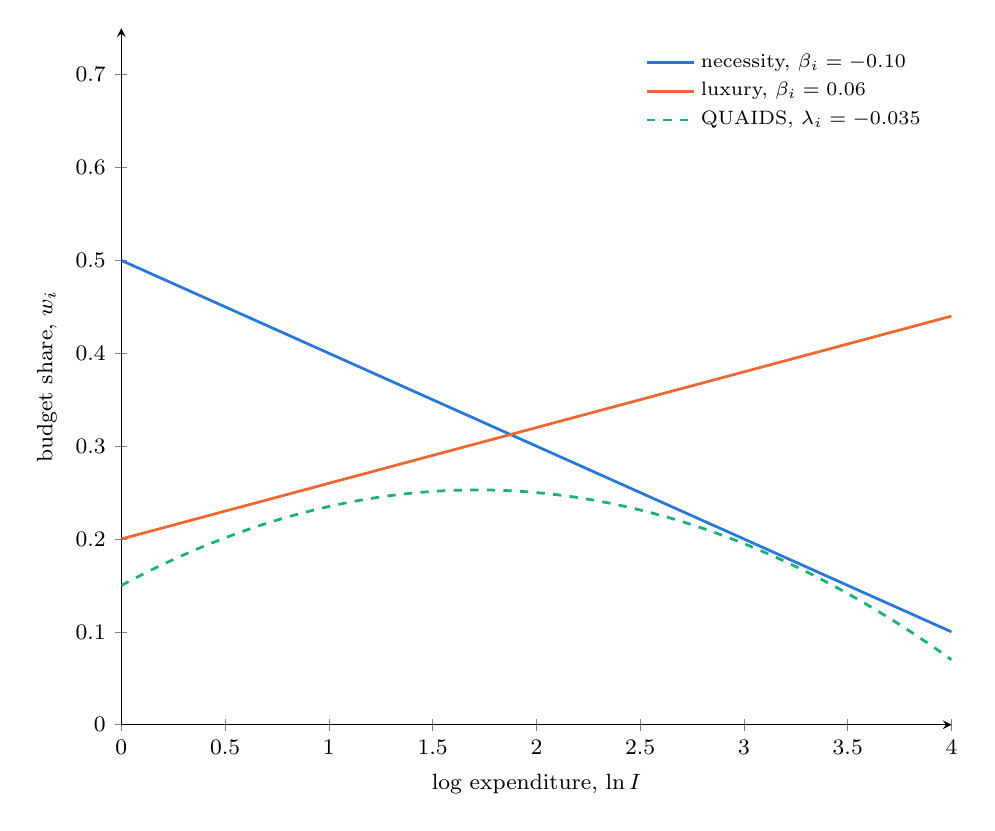
\begin{tikzpicture}
\begin{axis}[
  width=\linewidth, height=0.86\linewidth,
  axis lines=left, xmin=0, xmax=4, ymin=0, ymax=0.75,
  xlabel={log expenditure, $\ln I$}, ylabel={budget share, $w_i$},
  every axis plot/.append style={line width=1pt},
  legend style={font=\scriptsize, draw=none, fill=none, at={(0.98,0.98)}, anchor=north east},
  legend cell align=left,
  tick label style={font=\footnotesize}, label style={font=\footnotesize}]
\addplot[c05p1blue, domain=0:4, samples=2] {0.5 - 0.10*x};
\addlegendentry{necessity, $\beta_i = -0.10$}
\addplot[c05p1orange, domain=0:4, samples=2] {0.2 + 0.06*x};
\addlegendentry{luxury, $\beta_i = 0.06$}
\addplot[c05p1aqua, dashed, domain=0:4, samples=80] {0.15 + 0.12*x - 0.035*x^2};
\addlegendentry{QUAIDS, $\lambda_i = -0.035$}
\end{axis}
\end{tikzpicture}
\caption{Budget shares}\label{fig:05-engel-shares}
\end{subfigure}\hfill
\begin{subfigure}[t]{0.485\textwidth}
\centering
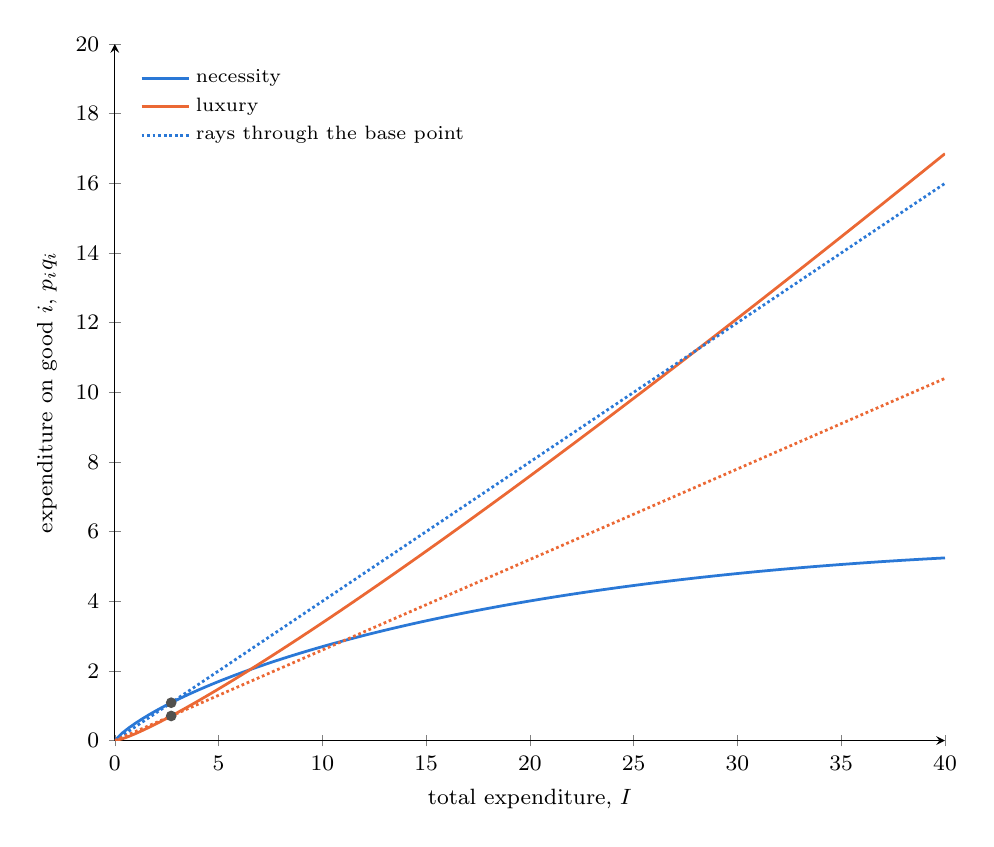
\begin{tikzpicture}
\begin{axis}[
  width=\linewidth, height=0.86\linewidth,
  axis lines=left, xmin=0, xmax=40, ymin=0, ymax=20,
  xlabel={total expenditure, $I$}, ylabel={expenditure on good $i$, $p_iq_i$},
  every axis plot/.append style={line width=1pt},
  legend style={font=\scriptsize, draw=none, fill=none, at={(0.02,0.98)}, anchor=north west},
  legend cell align=left,
  tick label style={font=\footnotesize}, label style={font=\footnotesize}]
\addplot[c05p1blue, domain=0.01:40, samples=120] {x*(0.5 - 0.10*ln(x))};
\addlegendentry{necessity}
\addplot[c05p1orange, domain=0.01:40, samples=120] {x*(0.2 + 0.06*ln(x))};
\addlegendentry{luxury}
\addplot[c05p1blue, densely dotted, domain=0:40, samples=2] {0.40*x};
\addlegendentry{rays through the base point}
\addplot[c05p1orange, densely dotted, domain=0:40, samples=2] {0.26*x};
\addplot[only marks, mark=*, mark size=1.4pt, c05p1gray] coordinates {(2.71828,1.08731) (2.71828,0.70675)};
\end{axis}
\end{tikzpicture}
\caption{Expenditure}\label{fig:05-engel-spending}
\end{subfigure}
\caption{Engel curves at unit prices. Panel (a) plots budget shares against $\ln I$ for good 1 of the running
example (a necessity, $w_1 = 0.5 - 0.10\ln I$), good 3 (a luxury, $w_3 = 0.2 + 0.06\ln I$), and an
illustrative QUAIDS good with $w = 0.15 + 0.12\ln I - 0.035(\ln I)^2$. The QUAIDS share rises until
$\ln I = \frac{0.12}{0.07} \approx 1.71$ and falls afterwards. Panel (b) plots the corresponding expenditures
$p_iq_i = w_iI$ for the two AIDS goods. The dotted rays are the homothetic Engel curves through the base point
$\ln I = 1$ (dots), where $w_1 = 0.40$ and $w_3 = 0.26$.}\label{fig:05-engel}
\end{figure}

\subsection{Why only almost ideal}\label{sec:05-aids-limits}

\citet[p.~312]{DeatonMuellbauer1980a} list six properties that together recommend the AIDS. It gives an
arbitrary first-order approximation to any demand system (\cref{prop:05-flexible}). It satisfies the axioms
of choice exactly, given the restrictions (\cref{prop:05-restrictions}). It aggregates over consumers without
invoking parallel linear Engel curves (\cref{sec:05-aggregation}). Its functional form is consistent with
household budget data (\cref{sec:05-engel}). It is simple to estimate and largely avoids nonlinear estimation
(\cref{sec:05-stone}). Finally, homogeneity and symmetry can be tested through linear restrictions on fixed
parameters (\cref{sec:05-testing}). The Rotterdam and translog models each possess some of these properties,
but neither possesses all of them at once. The authors themselves add that the system, particularly in its
simple static form, is not to be regarded as ``a fully satisfactory explanation of consumers' behavior''
\citep[p.~312]{DeatonMuellbauer1980a}.

The system falls short of the ideal in five ways.

\emph{Concavity is not guaranteed.} By \cref{prop:05-negativity}, negativity depends on the data point and
cannot be imposed by linear restrictions. Estimated systems often violate it at some observations. At unit
prices the running example is concave over the whole range of $\ln I$ in which all its shares lie in
$[0, 1]$, but this must be checked for every estimate.

\emph{Fitted shares can leave the unit interval.} Shares are linear in $\ln I$ and quadratic in $\ln p$, and
these variables are unbounded. For extreme prices or incomes the fitted shares become negative or exceed one, and the cost
function then ceases to be a valid expenditure function. In the running example at unit prices, the share of
good 1 is $0.5 - 0.10\ln I$, which turns negative above $\ln I = 5$. The share of good 3 turns negative below
$\ln I = -\frac{0.2}{0.06} \approx -3.33$. The appendix of \citet[p.~324]{DeatonMuellbauer1980a} derives the
corresponding restrictions on the admissible region of incomes and prices for the PIGLOG class.

\emph{There are many parameters.} The matrix $\Gamma$ has $J^2$ elements. Symmetry leaves
$\frac{J(J+1)}{2}$, and homogeneity removes $J$ more, leaving
\begin{equation}\label{eq:05-param-count}
\frac{J(J+1)}{2} - J = \frac{J(J-1)}{2}
\end{equation}
free price coefficients, about $\frac{1}{2}J^2$. Adding up then determines the last row of $\Gamma$ from the
others, and the $\alpha_i$ and $\beta_i$ add $2(J - 1)$ free parameters, plus $\alpha_0$. With $J = 8$
groups the count gives 28 free $\gamma_{ij}$ and 14 free $\alpha_i$ and $\beta_i$, the numbers that
\citet[p.~318]{DeatonMuellbauer1980a} report for their British application (\cref{sec:05-dm-application}).
With $J = 100$ products the count of $\gamma$'s is 4{,}950. \citet[p.~315]{DeatonMuellbauer1980a} suggest
setting individual $\gamma_{ij}$ to zero when theory or evidence supports it. The share of each good in such a
pair is then independent of the other's price at constant real expenditure. Setting every $\gamma_{ij}$
to zero is too strong. The resulting model, $w_i = \alpha_i + \beta_i\ln\frac{I}{\mathbf{P}}$, was tested and
rejected by \citet{Deaton1978}. The restrictions of \citet{ChaudhuriGoldbergJia2006} in \cref{sec:05-cgj}
follow the middle path.

\emph{Engel curves have rank two.} Shares are linear in $\ln I$, so a good cannot switch from luxury to
necessity as income grows. QUAIDS (\cref{prop:05-quaids}) relaxes this.

\emph{The choke price can be finite.} When the own share falls with $\ln p_i$, the demand for the good reaches
zero at a finite price. This is not automatic. With $\beta_i = 0$ it requires $\gamma_{ii} < 0$. The food
equation of \cref{tab:05-dm-table1} has $\gamma_{11} = 0.186$, and there the food share rises with the food
price. In the running example, holding the other prices at one and income at $\ln I = 1$,
the share of good 3 falls to zero at $p_3 \approx 4.10$. A finite virtual price lets the estimated own and
cross effects determine the value of a good, instead of the functional form alone (\cref{sec:05-three-systems}). It also means that
welfare calculations extrapolate the estimated demand curve well beyond the observed prices.
\Cref{sec:05-welfare-virtual} develops both sides of this feature.

Most of these limits are the price of a system that is linear enough to estimate and flexible enough to
test. The rest of the chapter shows how applied work lives with them: by aggregating goods into groups and
budgeting in stages, by instrumenting prices, and by checking curvature and extrapolation explicitly.
